\documentclass{beamer}
\usepackage{graphicx}
\usepackage{hyperref}
\usepackage[sorting=none]{biblatex}
\usepackage[font=small,skip=0pt]{caption}
\bibliography{refs}
\renewcommand{\footnotesize}{\fontsize{6pt}{6pt}\selectfont}
\usetheme{Madrid}
\usecolortheme{beaver}
\titlegraphic{
\includegraphics[width=2.5cm]{logo.png}}
\title[High Harmonic Generation]{High Harmonic Generation in Laser Plasma Interaction}
\date{}
\institute[IITD]{\large Indian Institute of Technology, Delhi}
\author[]{Kulwinder Kaur (2021PHS7190)\\ Harikesh Kushwaha (2021PHS7181)\\[3mm]Adviser: Prof. Vikrant Saxena}
\vspace{0cm}
\begin{document}
\maketitle

\begin{frame}{Introduction}
    \frametitle{Introduction}
    \small
    Ultra high light intensity interactions with matter provide an opportunity to investigate new physical phenomena that have yet to be explored or have been only minimally explored in laboratory settings.
    \begin{itemize}
        \item Intensity of $10^{23} \; W/cm^{2}$ has been reached experimentally.\footnote{\textit{Henri Vincenti} 10.1103/physrevlett.123.105001}
        \item QED at $I = 10^{25}W/cm^{2}$. Schwinger field at $I = 10^{29}W/cm^{2}$.\footnote{\textit{Jin Woo Yoon et al} 10.1364/OPTICA.420520}
        \item Plasma is overdense if $\omega<\omega_p$.
        \item Harmonics are generated by interaction of laser with overdense plasma.
    \end{itemize}
    \begin{minipage}[h]{0.48\linewidth}
        \centering
        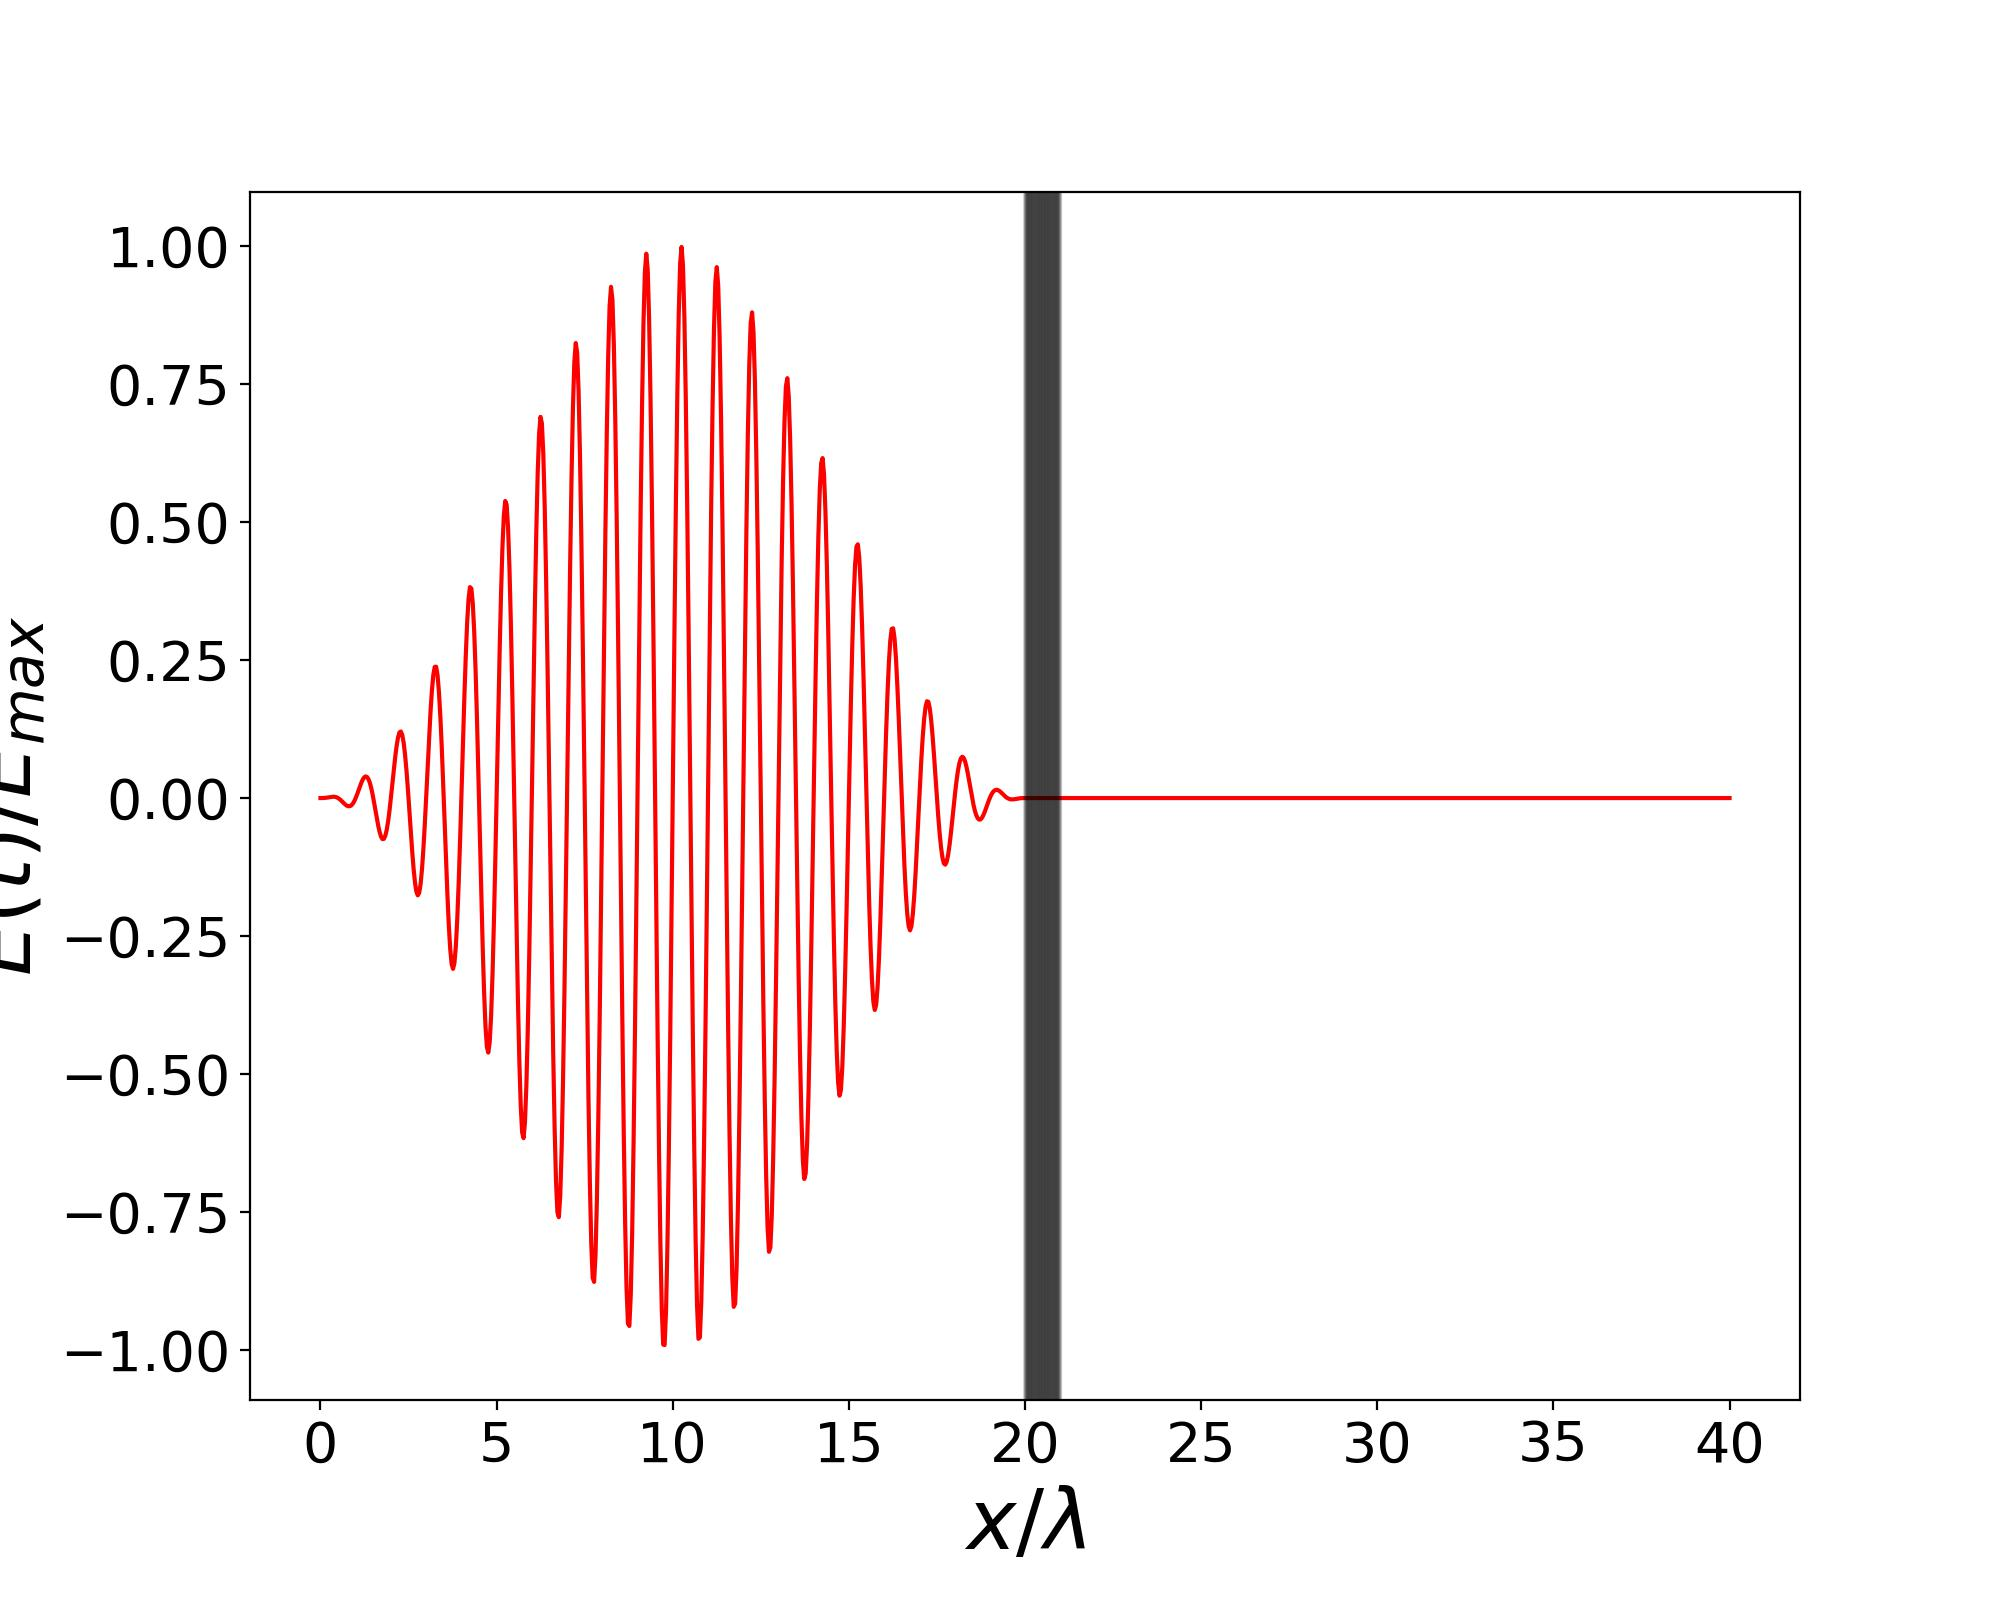
\includegraphics[width=0.9\textwidth, height=0.42\textheight]{images/field.jpg}
        \label{fig:field}
    \end{minipage}
    \begin{minipage}[h]{0.48\linewidth}
        \begin{figure}
            \centering
            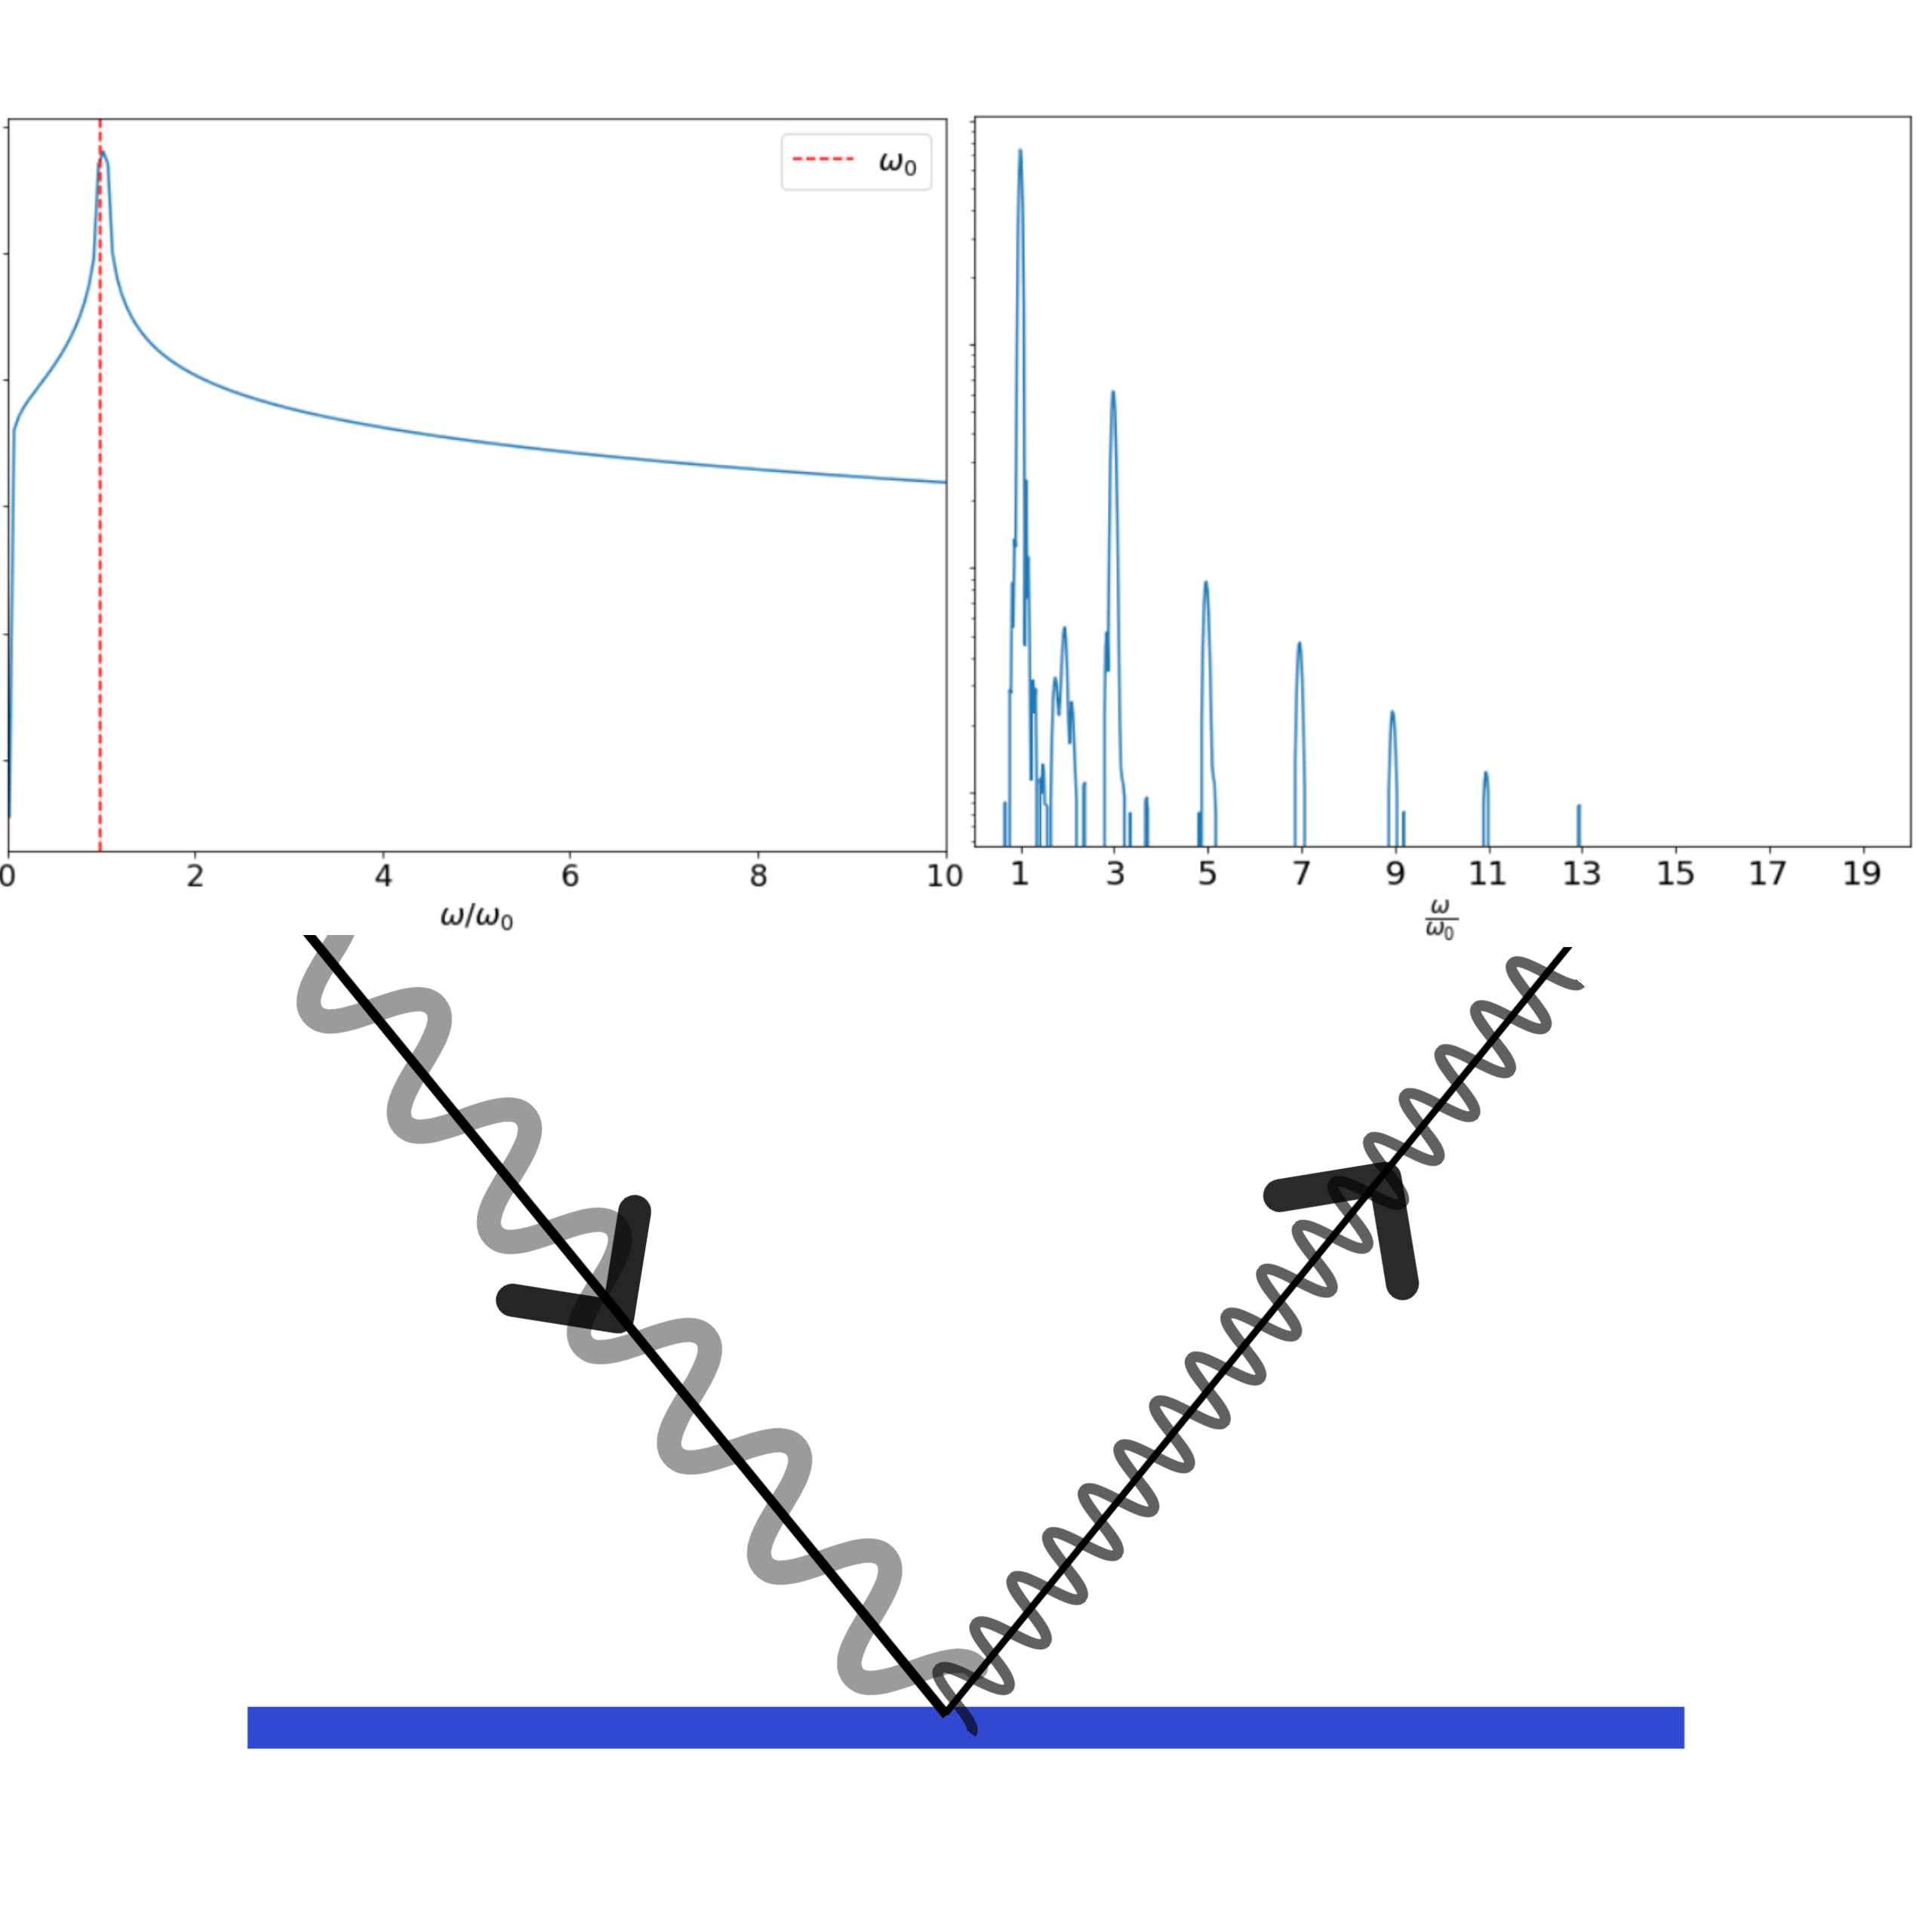
\includegraphics[width=0.9\textwidth, height=0.42\textheight]{images/harmonics.png}
            \label{fig:harmonics}
        \end{figure}
    \end{minipage}
\end{frame}

\begin{frame}
    \frametitle{Summary of Work Done in the Previous Semester}
    \small
    \begin{itemize}
        \item Interaction of intense laser pulse with overdense and underdense plasma
        \item Change in effective critical density of plasma for relativistic laser pulse
        \item The oscillations of plasma surface increases with increase in intensity and surface oscillations have even harmonics.
              %   \begin{itemize}
              %   \item Oscillations increases with increase in intensity
              %   \item Surface oscillations have even harmonics
              %   \end{itemize}
        \item Study of high harmonics generation in normal incidence
              \begin{itemize}
                  \item Only odd harmonics are generated
                        %   \item A resonance at $n_0/n_c=4$ is observed
                  \item Increasing intensity and pulse duration increases number of harmonics
                  \item No effect due to envelopes
              \end{itemize}
        \item Study of high harmonics generation in oblique incidence
              \begin{itemize}
                  \item For p-polarization $E_x$ gives even harmonics and $E_y$ gives odd harmonics
                        %   \item Both odd and even harmonics are generated.
                  \item For s-polarization $E_z$ gives odd harmonics and $E_x$ gives even harmonics
                        %   \item For p-polarization $E_x$ gives even harmonics and $E_y$ gives odd harmonics
              \end{itemize}
    \end{itemize}

    \textbf{What Now?}
    \begin{itemize}
        \item Effect of pre-plasma
        \item Effect of Super Gaussian (SG) envelope
        \item 2D simulation for oblique incidence and different polarization
    \end{itemize}
\end{frame}
\begin{frame}
    \small
    \frametitle{PIC Algorithm}
    PIC is a numerical approach that simulates a collection of particles that interact via external and self-induced electromagnetic fields.
    % \cite{suciu}
    \begin{figure}
        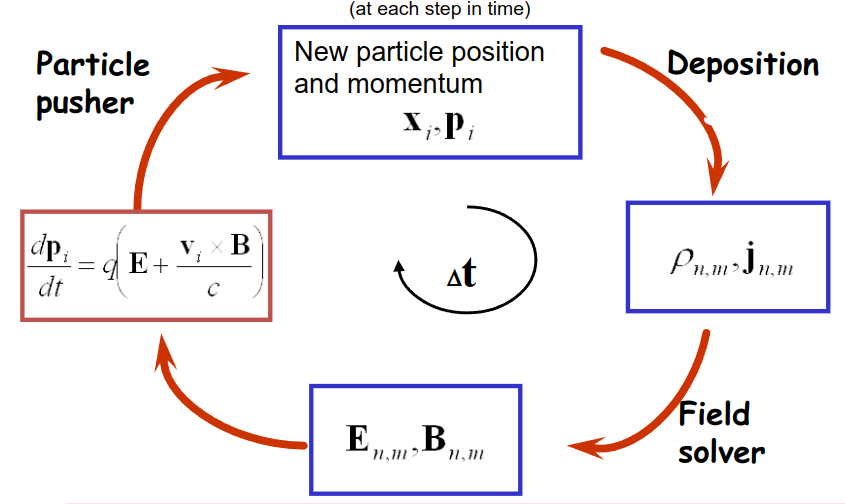
\includegraphics[width=10cm, height=6cm]{images/PIC.png}
        \centering
        % \caption{The PIC Cycle}
    \end{figure}

\end{frame}

\begin{frame}
    \frametitle{Simulation Details: 1D}
    \small
    We want to study the effect of super Gaussian envelope on the generated high harmonics. We performed some simulations in 1D3V. Here are some parameters:

    \begin{minipage}[t]{0.48\linewidth}
        \begin{itemize}
            \item Particles per cell: 100
            \item Number of cells: 16000
            \item Wavelength $\lambda_l = 1 \mu m$
            \item Pulse duration $= 20 \tau$ ($\tau\approx 3.3 fs$)
            \item Simulation time $= 40 \tau$
            \item Intensity of laser for $a_0 = 0.5$ is $I = 3.425 \times 10^{17} W/cm^2$
            \item The density to critical density ratio is $n_0/n_c = 4$
        \end{itemize}
        Previously, we performed simulations with p- and s-polarized laser incidence at oblique angle in 1D.
    \end{minipage}
    \begin{minipage}[t]{0.48\linewidth}
        \begin{figure}
            \centering
            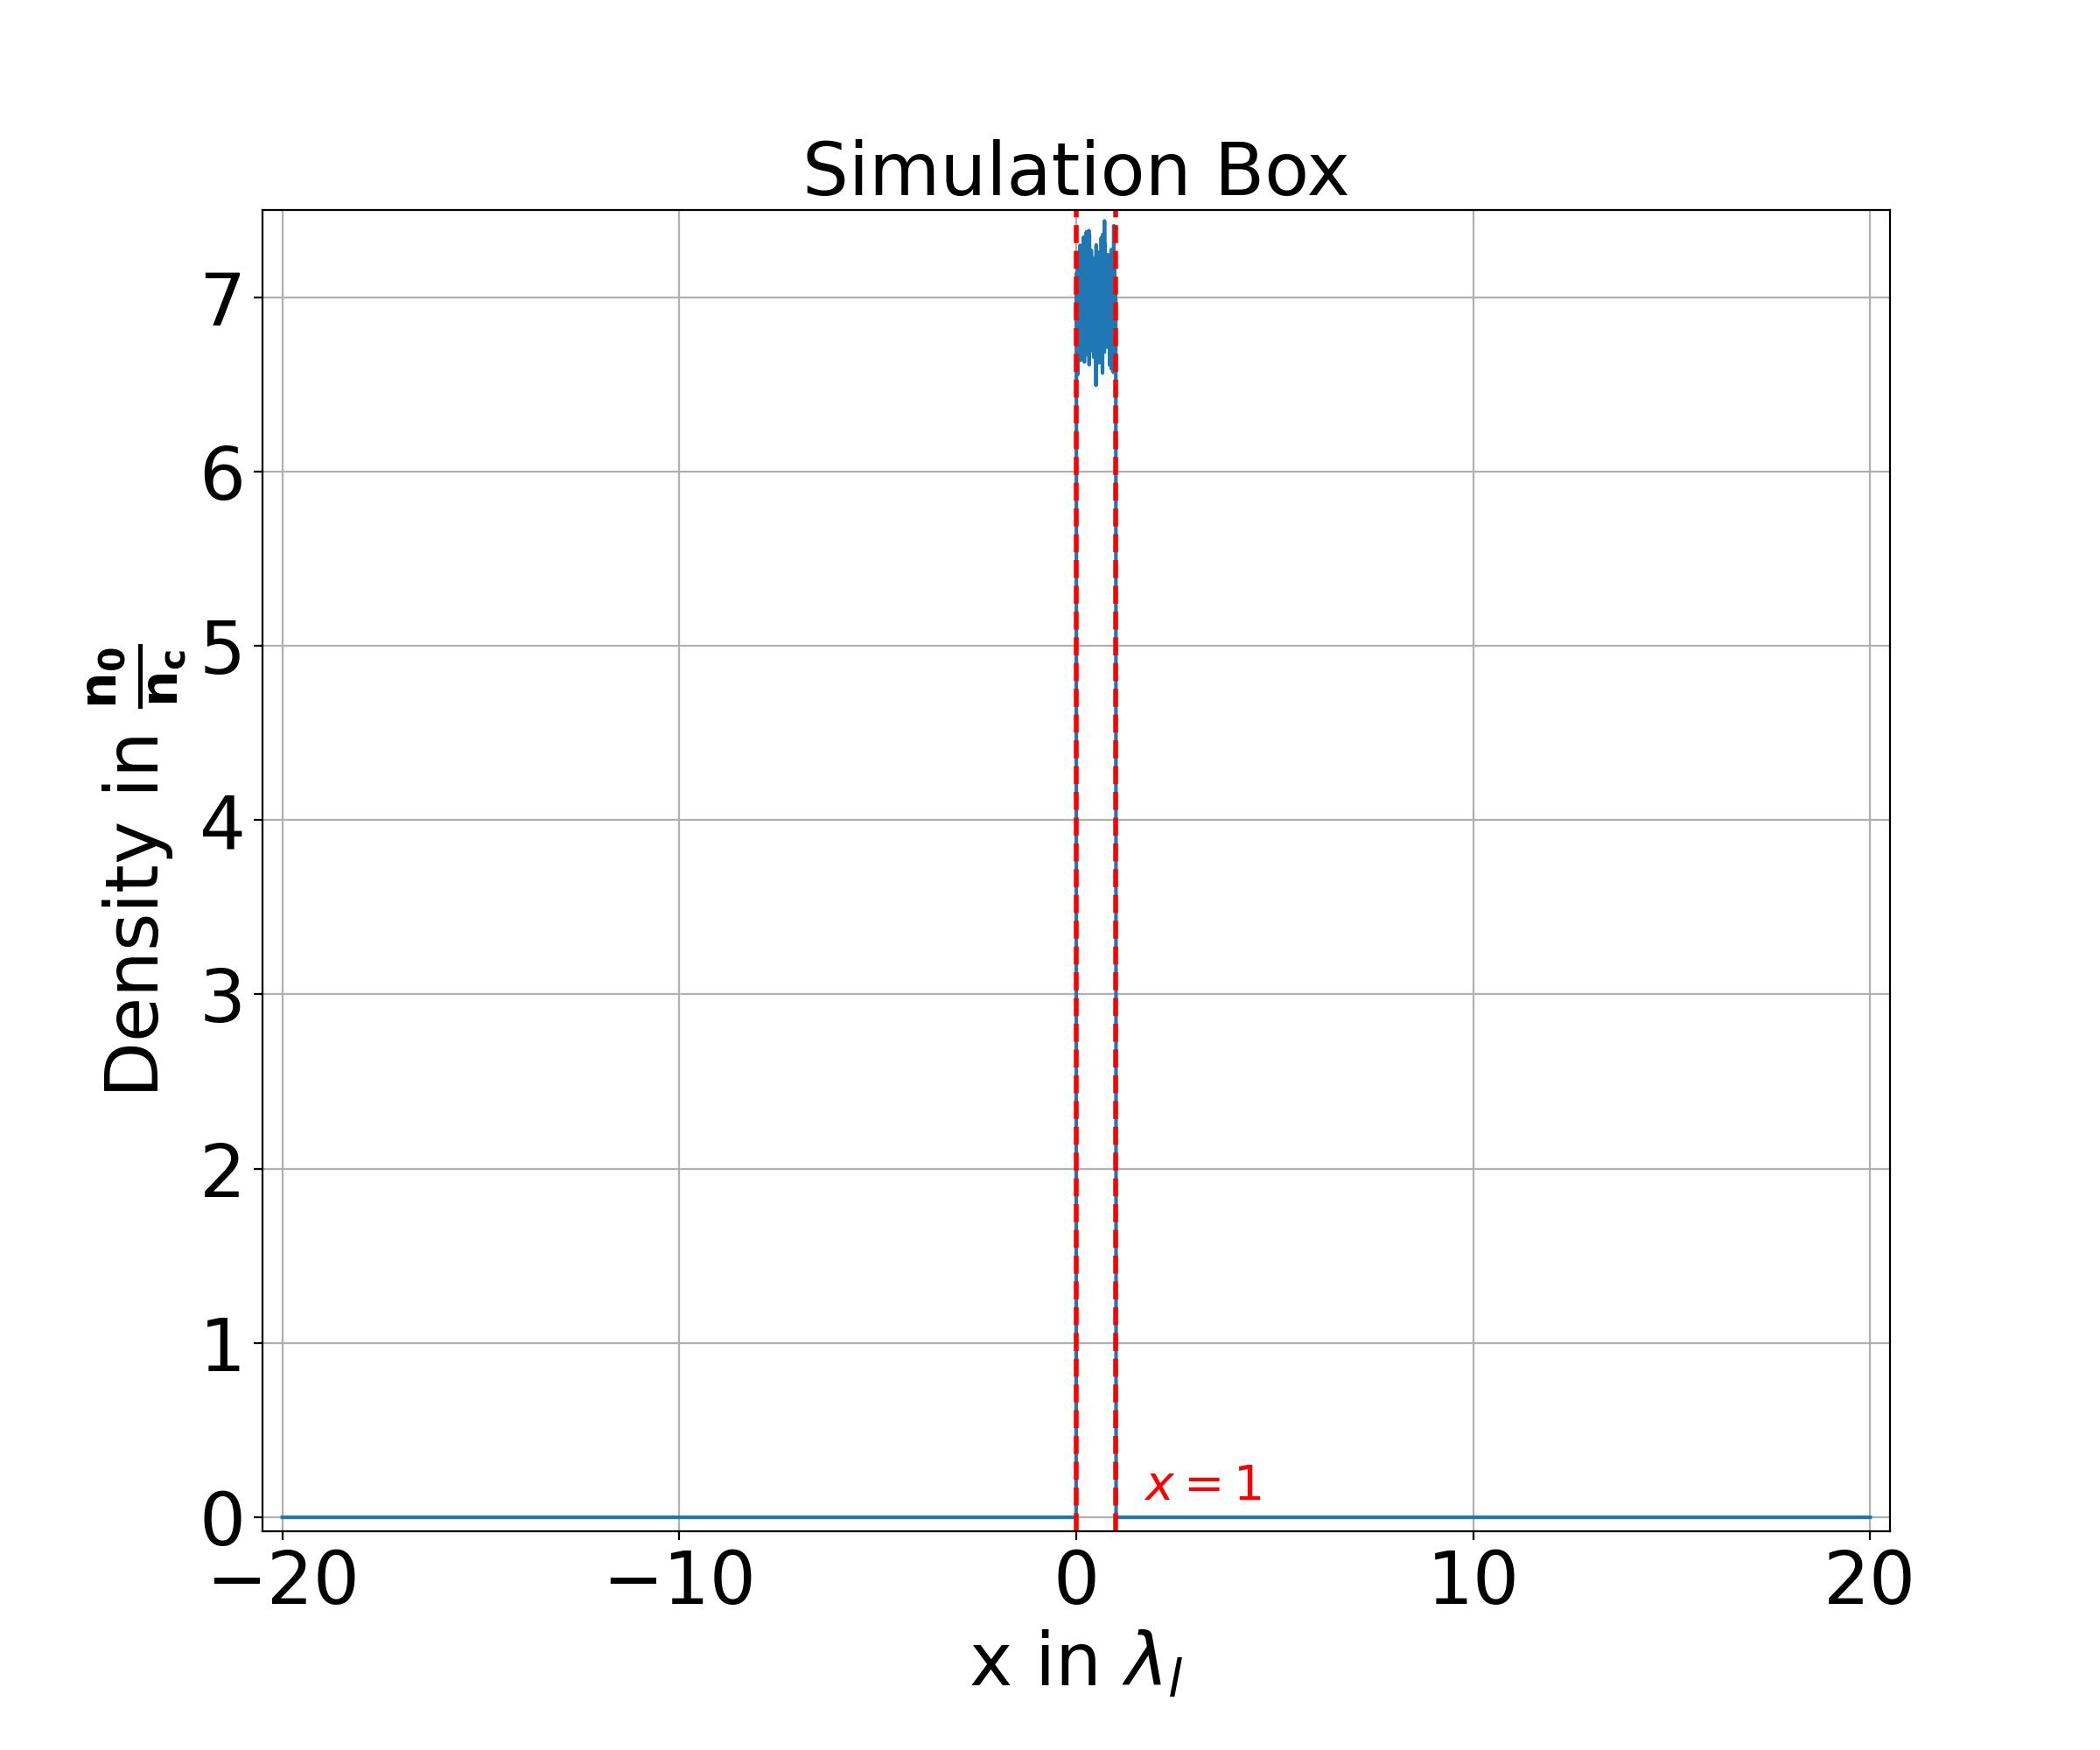
\includegraphics[width=1.0\textwidth, height=0.62\textheight]{images/plasma.jpg}
            \label{fig:plasma}
        \end{figure}
    \end{minipage}
\end{frame}

\begin{frame}
    \frametitle{Oblique Incidence: Transformations}
    \small
    \begin{itemize}
        \item We follow Bourdier\footnote{\textit{Bourdier,A. } 10 . 1063 / 1.864355} to make a transformation which lets us simulate oblique incidence in 1D.
    \end{itemize}
    \begin{minipage}[t]{0.35\linewidth}
        \begin{align*}
            \begin{split}
                &\text{For p-polarization}\\
                \mathbf{E}_L  & = E_0(-\sin\alpha \hat{x} + \cos\alpha \hat{y}) \\
                \mathbf{E}_M  & = E_0\cos\alpha \hat{y}                         \\
                c\mathbf{B}_L & = E_0\hat{z}                                    \\
                c\mathbf{B}_M & = E_0\cos\alpha \hat{z}\\
                &\text{For s-polarization}\\
                \mathbf{E}_L & = E_0\hat{z}                                    \\
                \mathbf{E}_M & = E_0\cos\alpha \hat{z}                        \\
                c\mathbf{B}_L & = E_0(\sin\alpha \hat{x} - \cos\alpha \hat{y}) \\
                c\mathbf{B}_M & = -E_0\cos\alpha \hat{y}
            \end{split}
        \end{align*}

    \end{minipage}
    \begin{minipage}[t]{0.60\linewidth}
        \begin{figure}
            \centering
            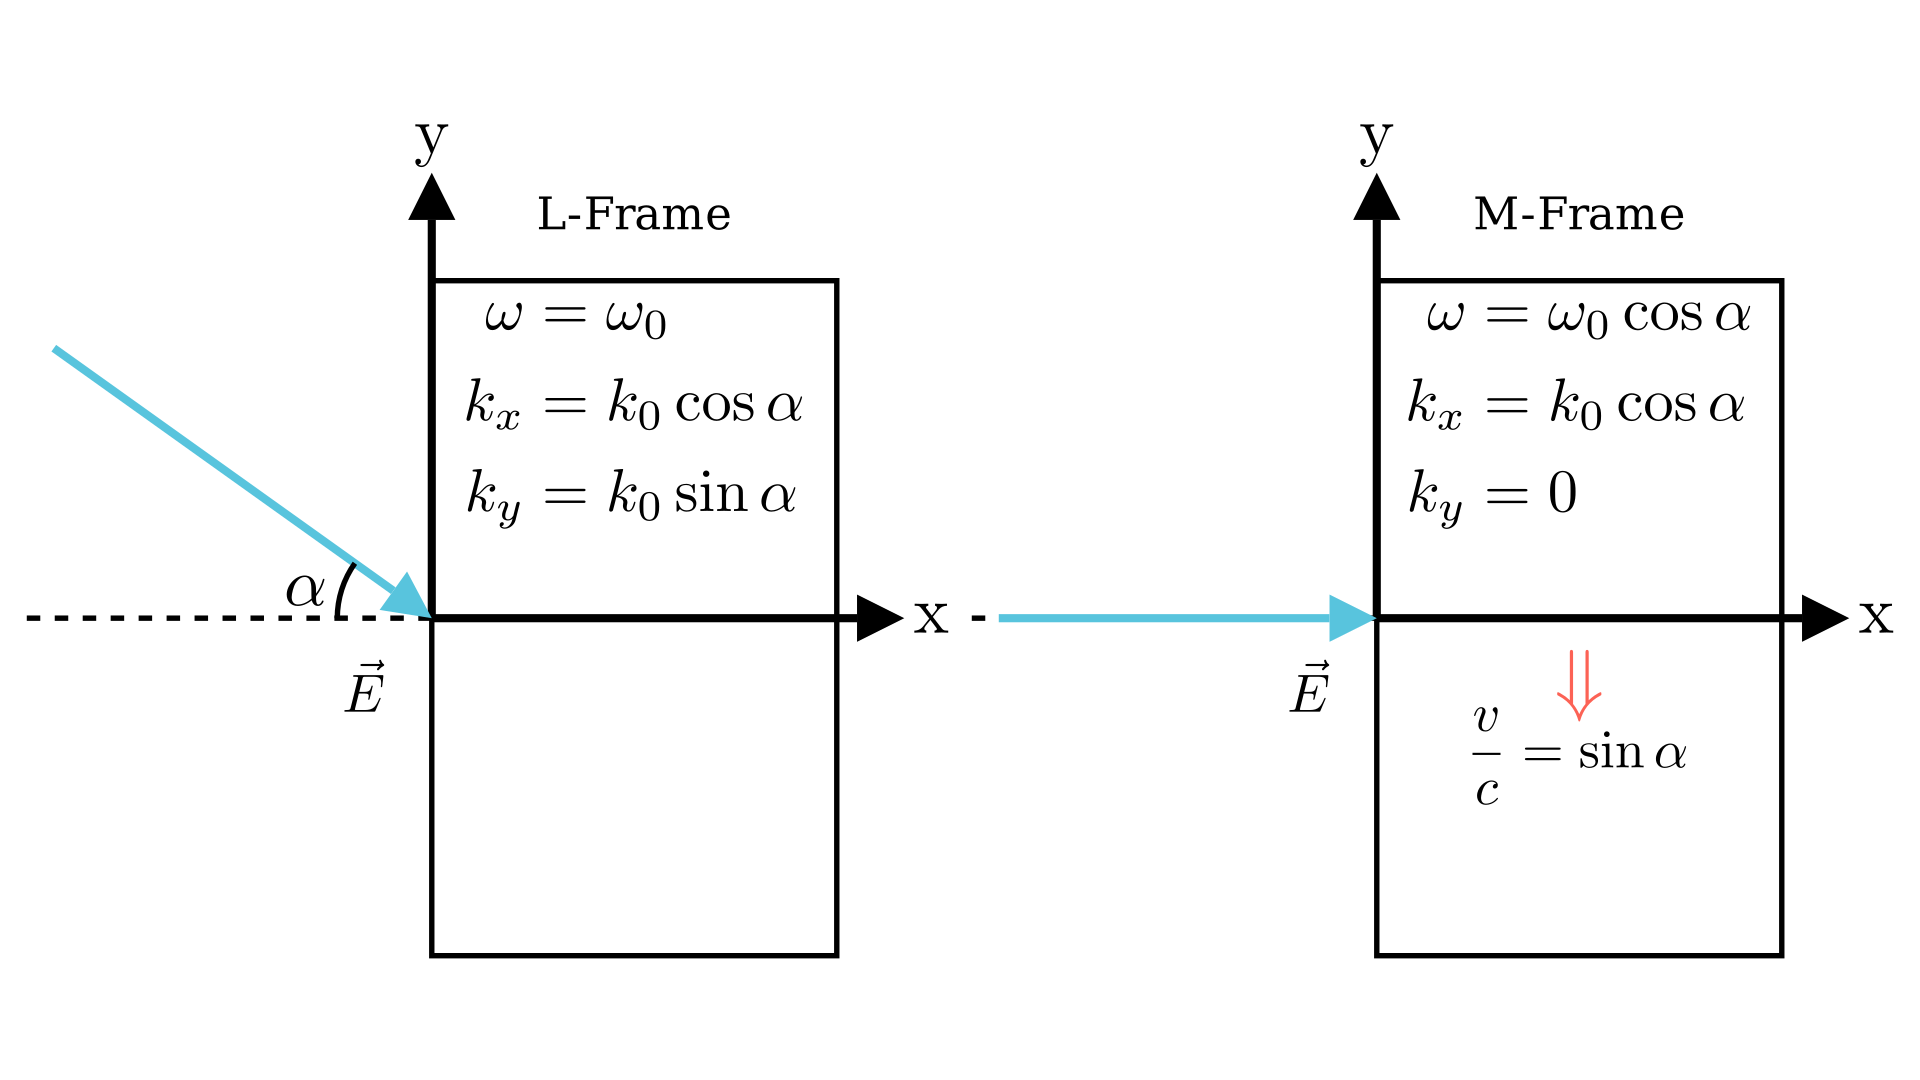
\includegraphics[width=1.0\textwidth, height=0.62\textheight]{images/frames.png}
            \label{fig:frames}
        \end{figure}
    \end{minipage}
\end{frame}

\begin{frame}
    \frametitle{p- and s- Polarized Laser: Selection Rule}
    \begin{minipage}[h]{0.18\linewidth}
        \small{p-Polarization}
        \tiny{
            \textbf{p-Polarized:}Even, Odd

            \textbf{s-Polarized:} None}
    \end{minipage}
    \begin{minipage}[h]{0.8\linewidth}
        \centering
        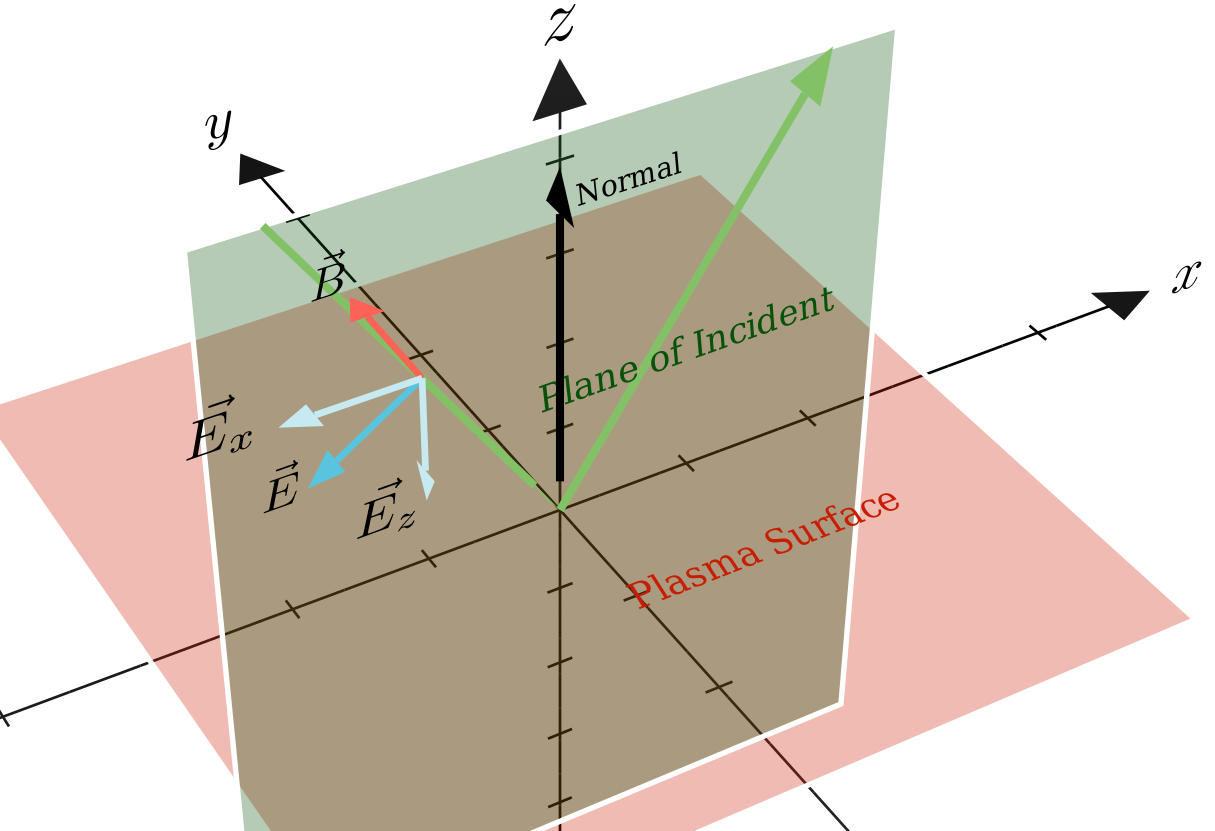
\includegraphics[width=0.9\textwidth, height=0.42\textheight]{images/p.png}
        \label{fig:p}
    \end{minipage}

    \begin{minipage}[h]{0.8\linewidth}
        \centering
        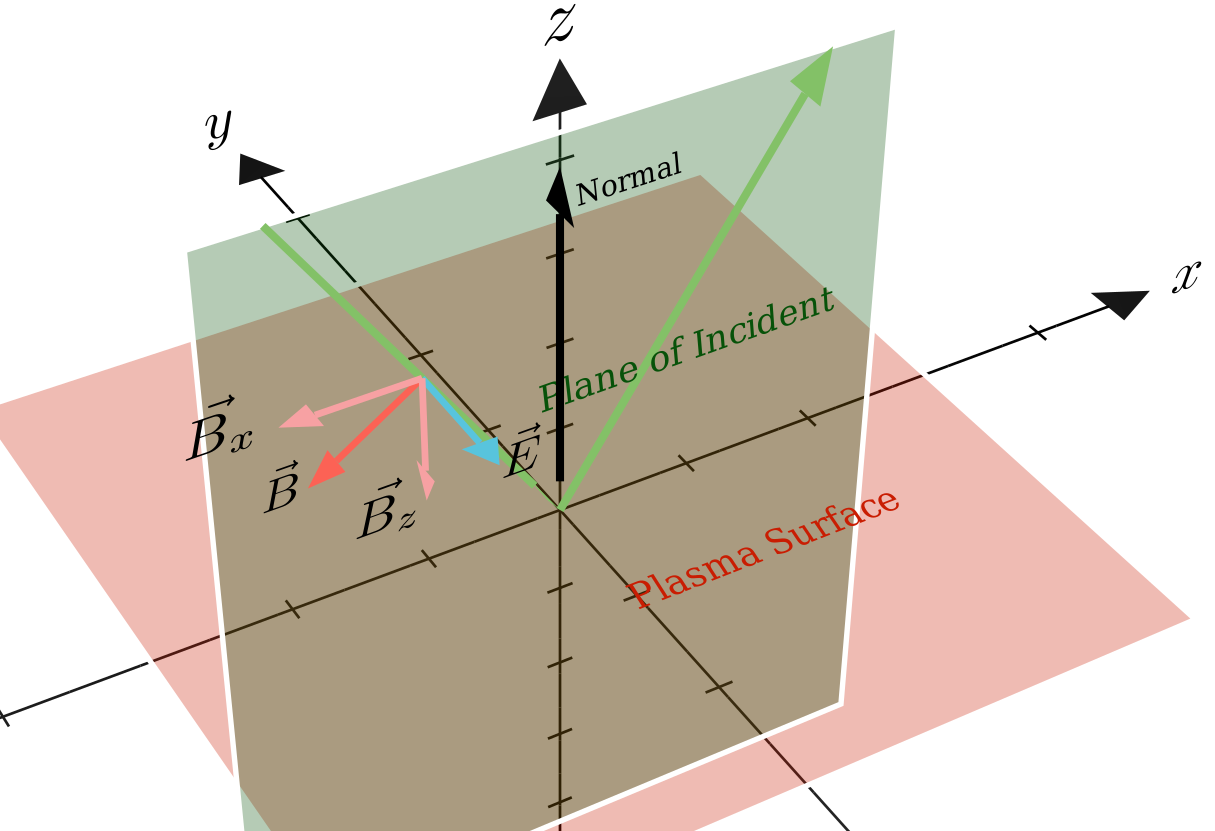
\includegraphics[width=0.9\textwidth, height=0.42\textheight]{images/s.png}
        \label{fig:s}
    \end{minipage}
    \begin{minipage}[h]{0.18\linewidth}
        \small{s-Polarization}
        \tiny{
            \textbf{p-Polarized:} Even

            \textbf{s-Polarized:} Odd}
    \end{minipage}

\end{frame}

\begin{frame}
    \frametitle{Results: Effect of  Pre-Plasma}
    \begin{minipage}[h]{0.48\linewidth}
        \centering
        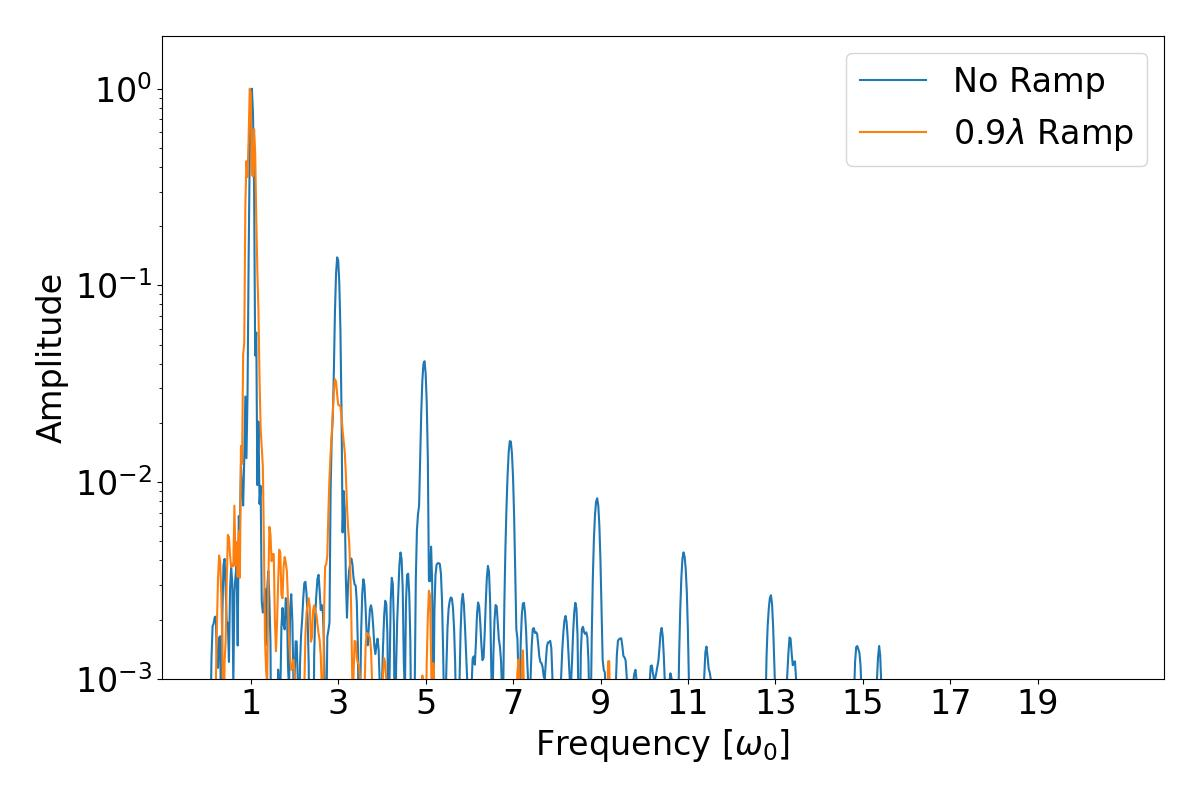
\includegraphics[width=1\textwidth, height=0.55\textheight]{images/ramp.jpg}
        \scriptsize{The spectrum of the reflected field with and without a pre-plasma. A suppression in the HHG amplitude is observed for case with pre-plasma.}
        \label{fig:ramp}
    \end{minipage}
    \begin{minipage}[h]{0.48\linewidth}
        \centering
        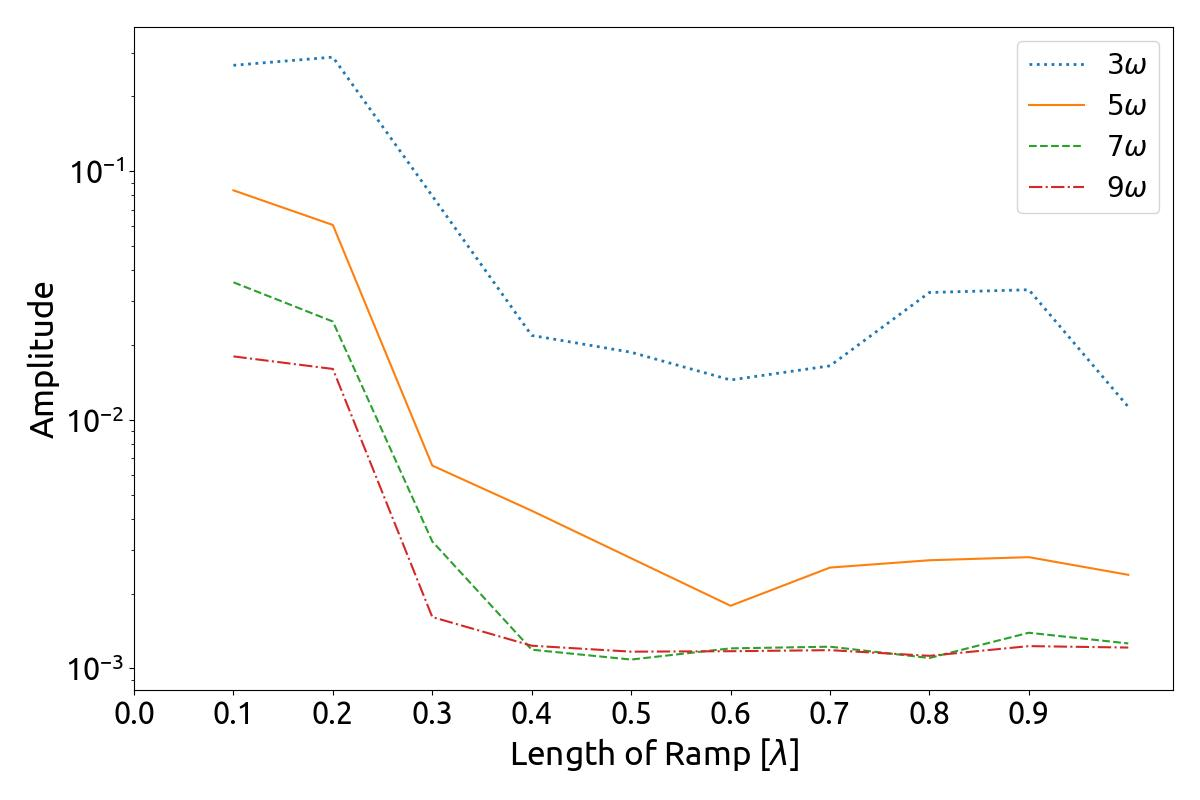
\includegraphics[width=1\textwidth, height=0.55\textheight]{images/ramp_7600.jpg}
        \scriptsize{The peak of different harmonics for different ramp. The figure shows that as the ramp length increases, the amplitudes of the harmonics decreases.}
        \label{fig:ramp-peaks}
    \end{minipage}
\end{frame}

\begin{frame}
    \frametitle{Results: Effect of  Pre-Plasma}
    \centering
    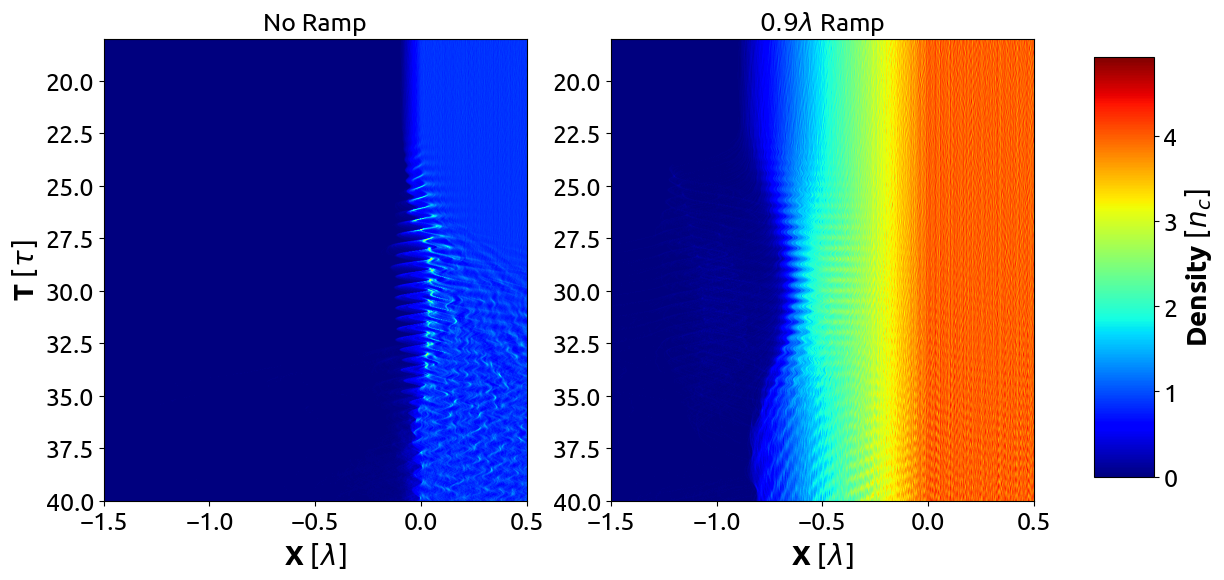
\includegraphics[width=1\textwidth]{images/ramp_d.png}
    \scriptsize{The laser is not able to interact with the main plasma and hence the efficiency of HHG is reduced.}
    \label{fig:ramp-density}
\end{frame}

\begin{frame}
    \frametitle{Results: SG Envelope}
    \begin{minipage}[h]{0.48\linewidth}
        \centering
        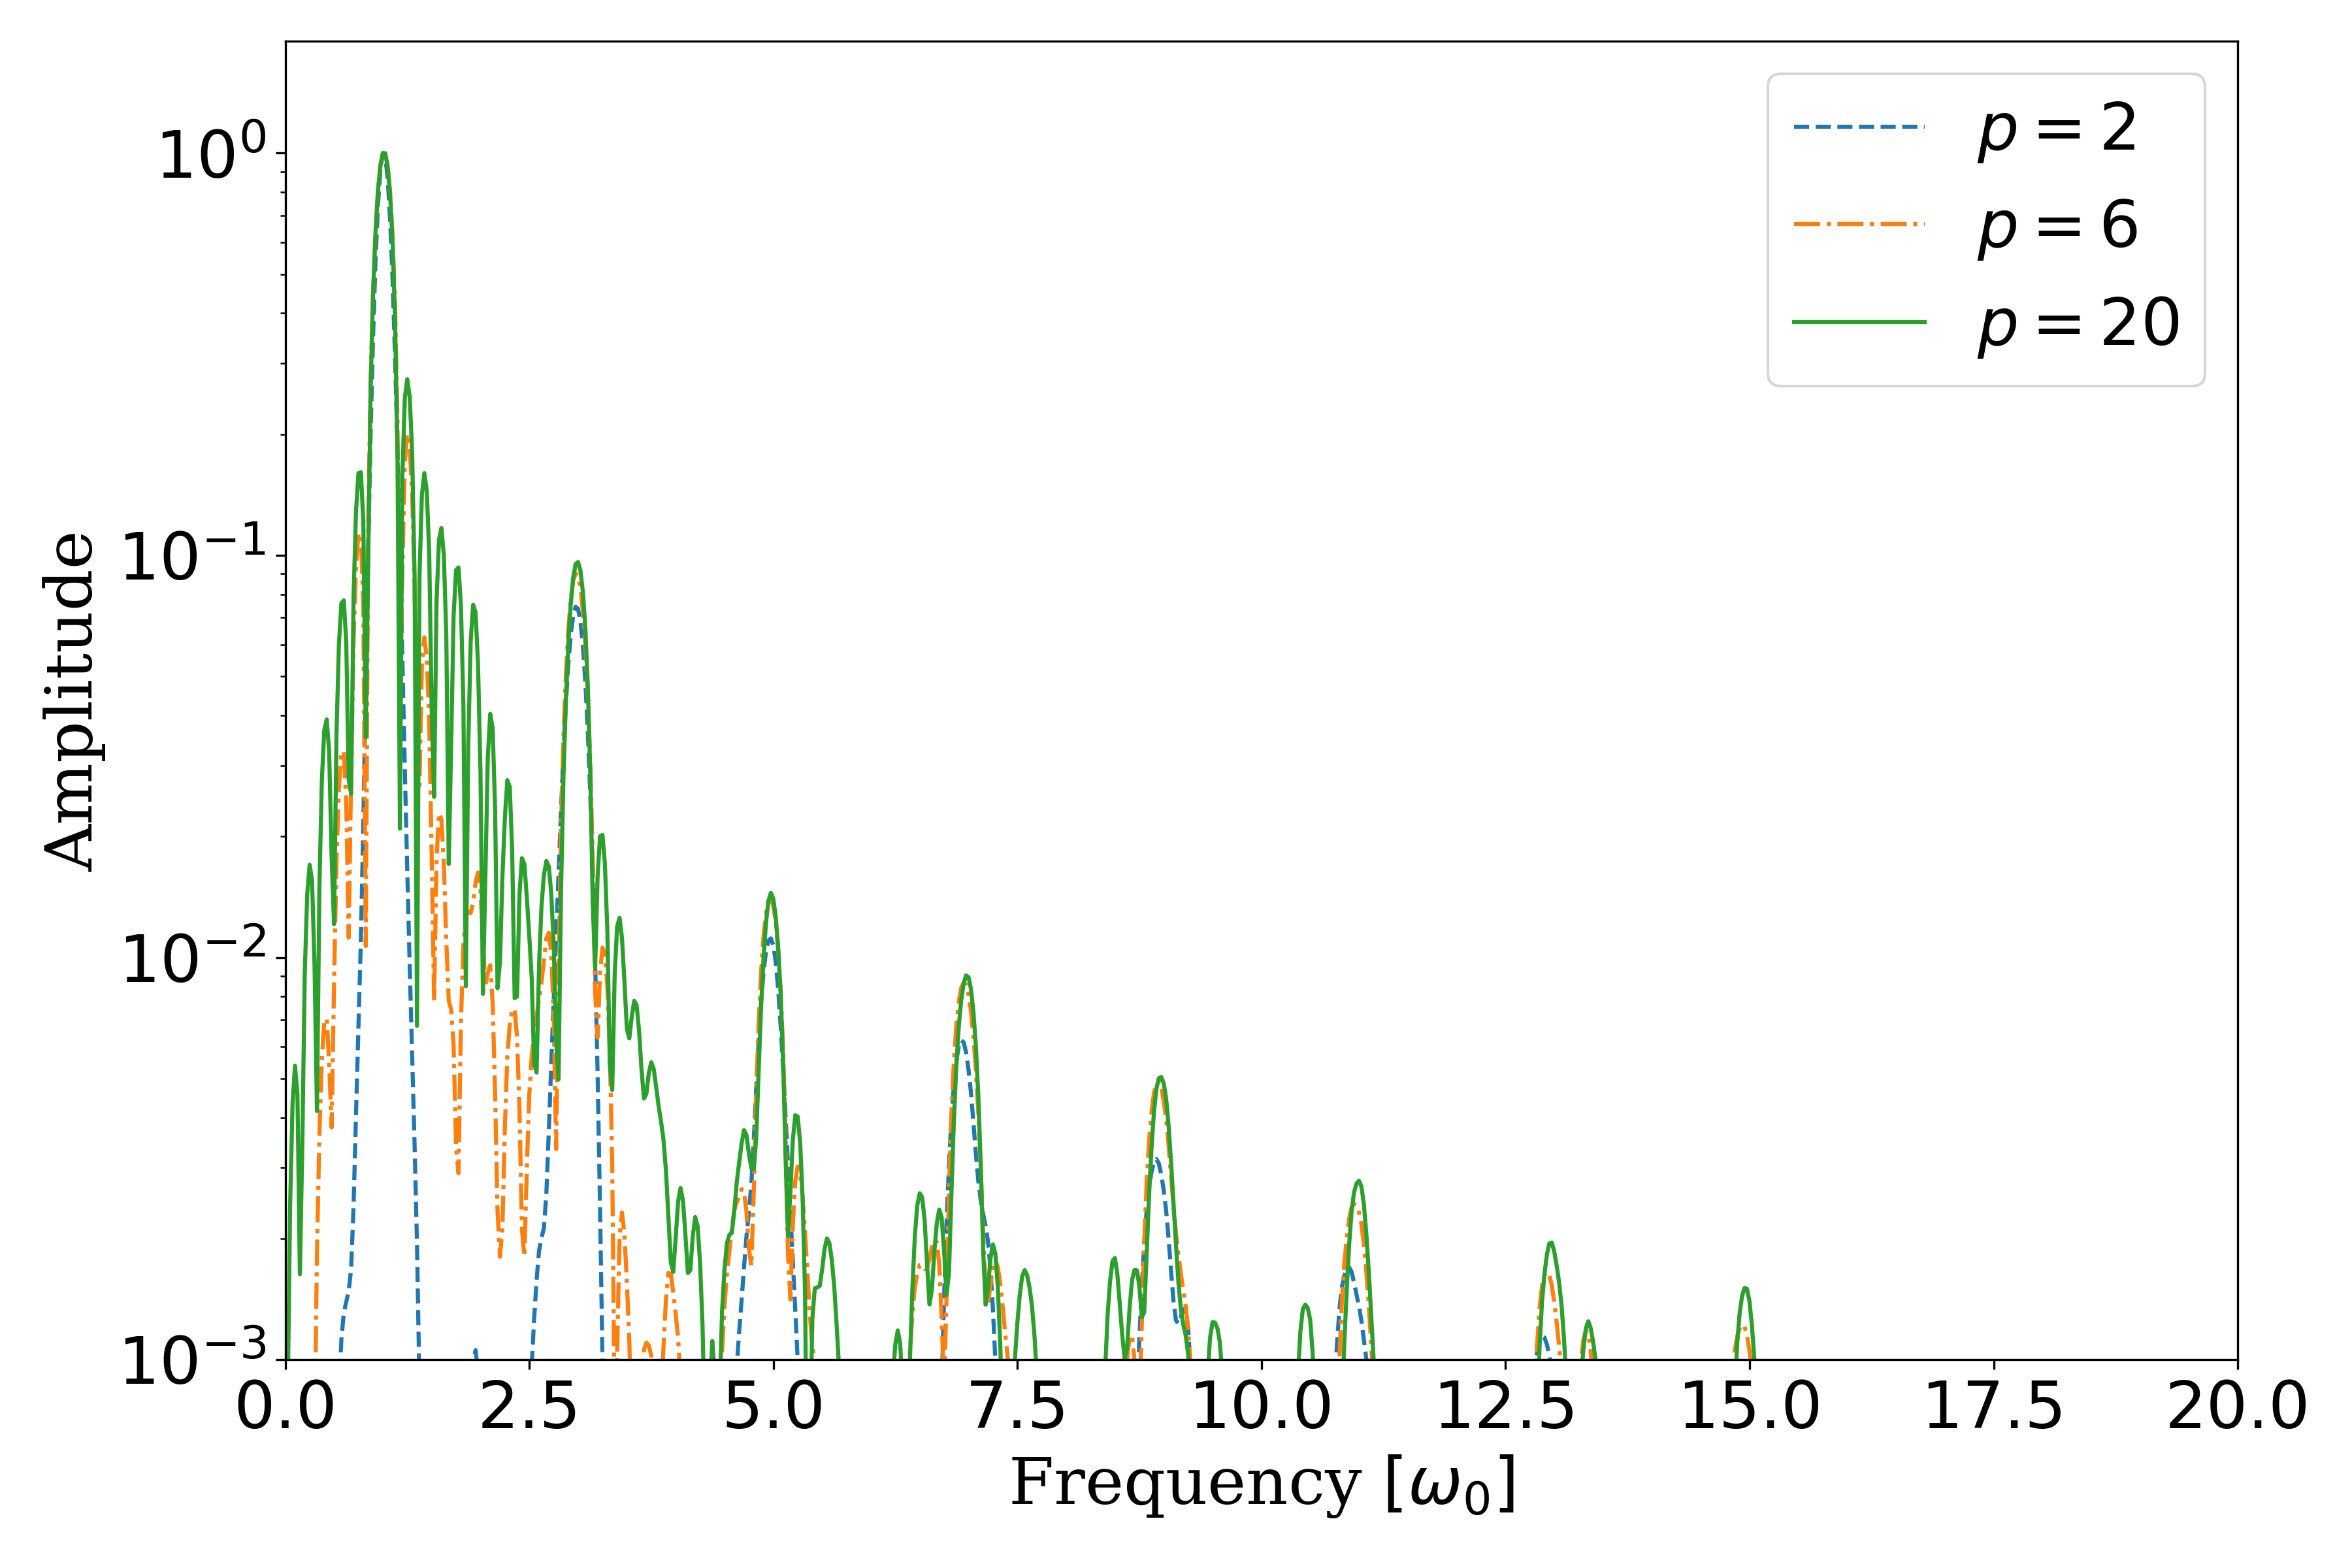
\includegraphics[width=1\textwidth, height=0.60\textheight]{images/SG_ffts_2-6-20.png}
        \scriptsize{The spectrum of SG envelopes with power 2,6, and 20 is shown in a single plot. A small increase in the peak amplitude is observed with increasing power.}
        \label{fig:sg-fft}
    \end{minipage}
    \begin{minipage}[h]{0.48\linewidth}
        \centering
        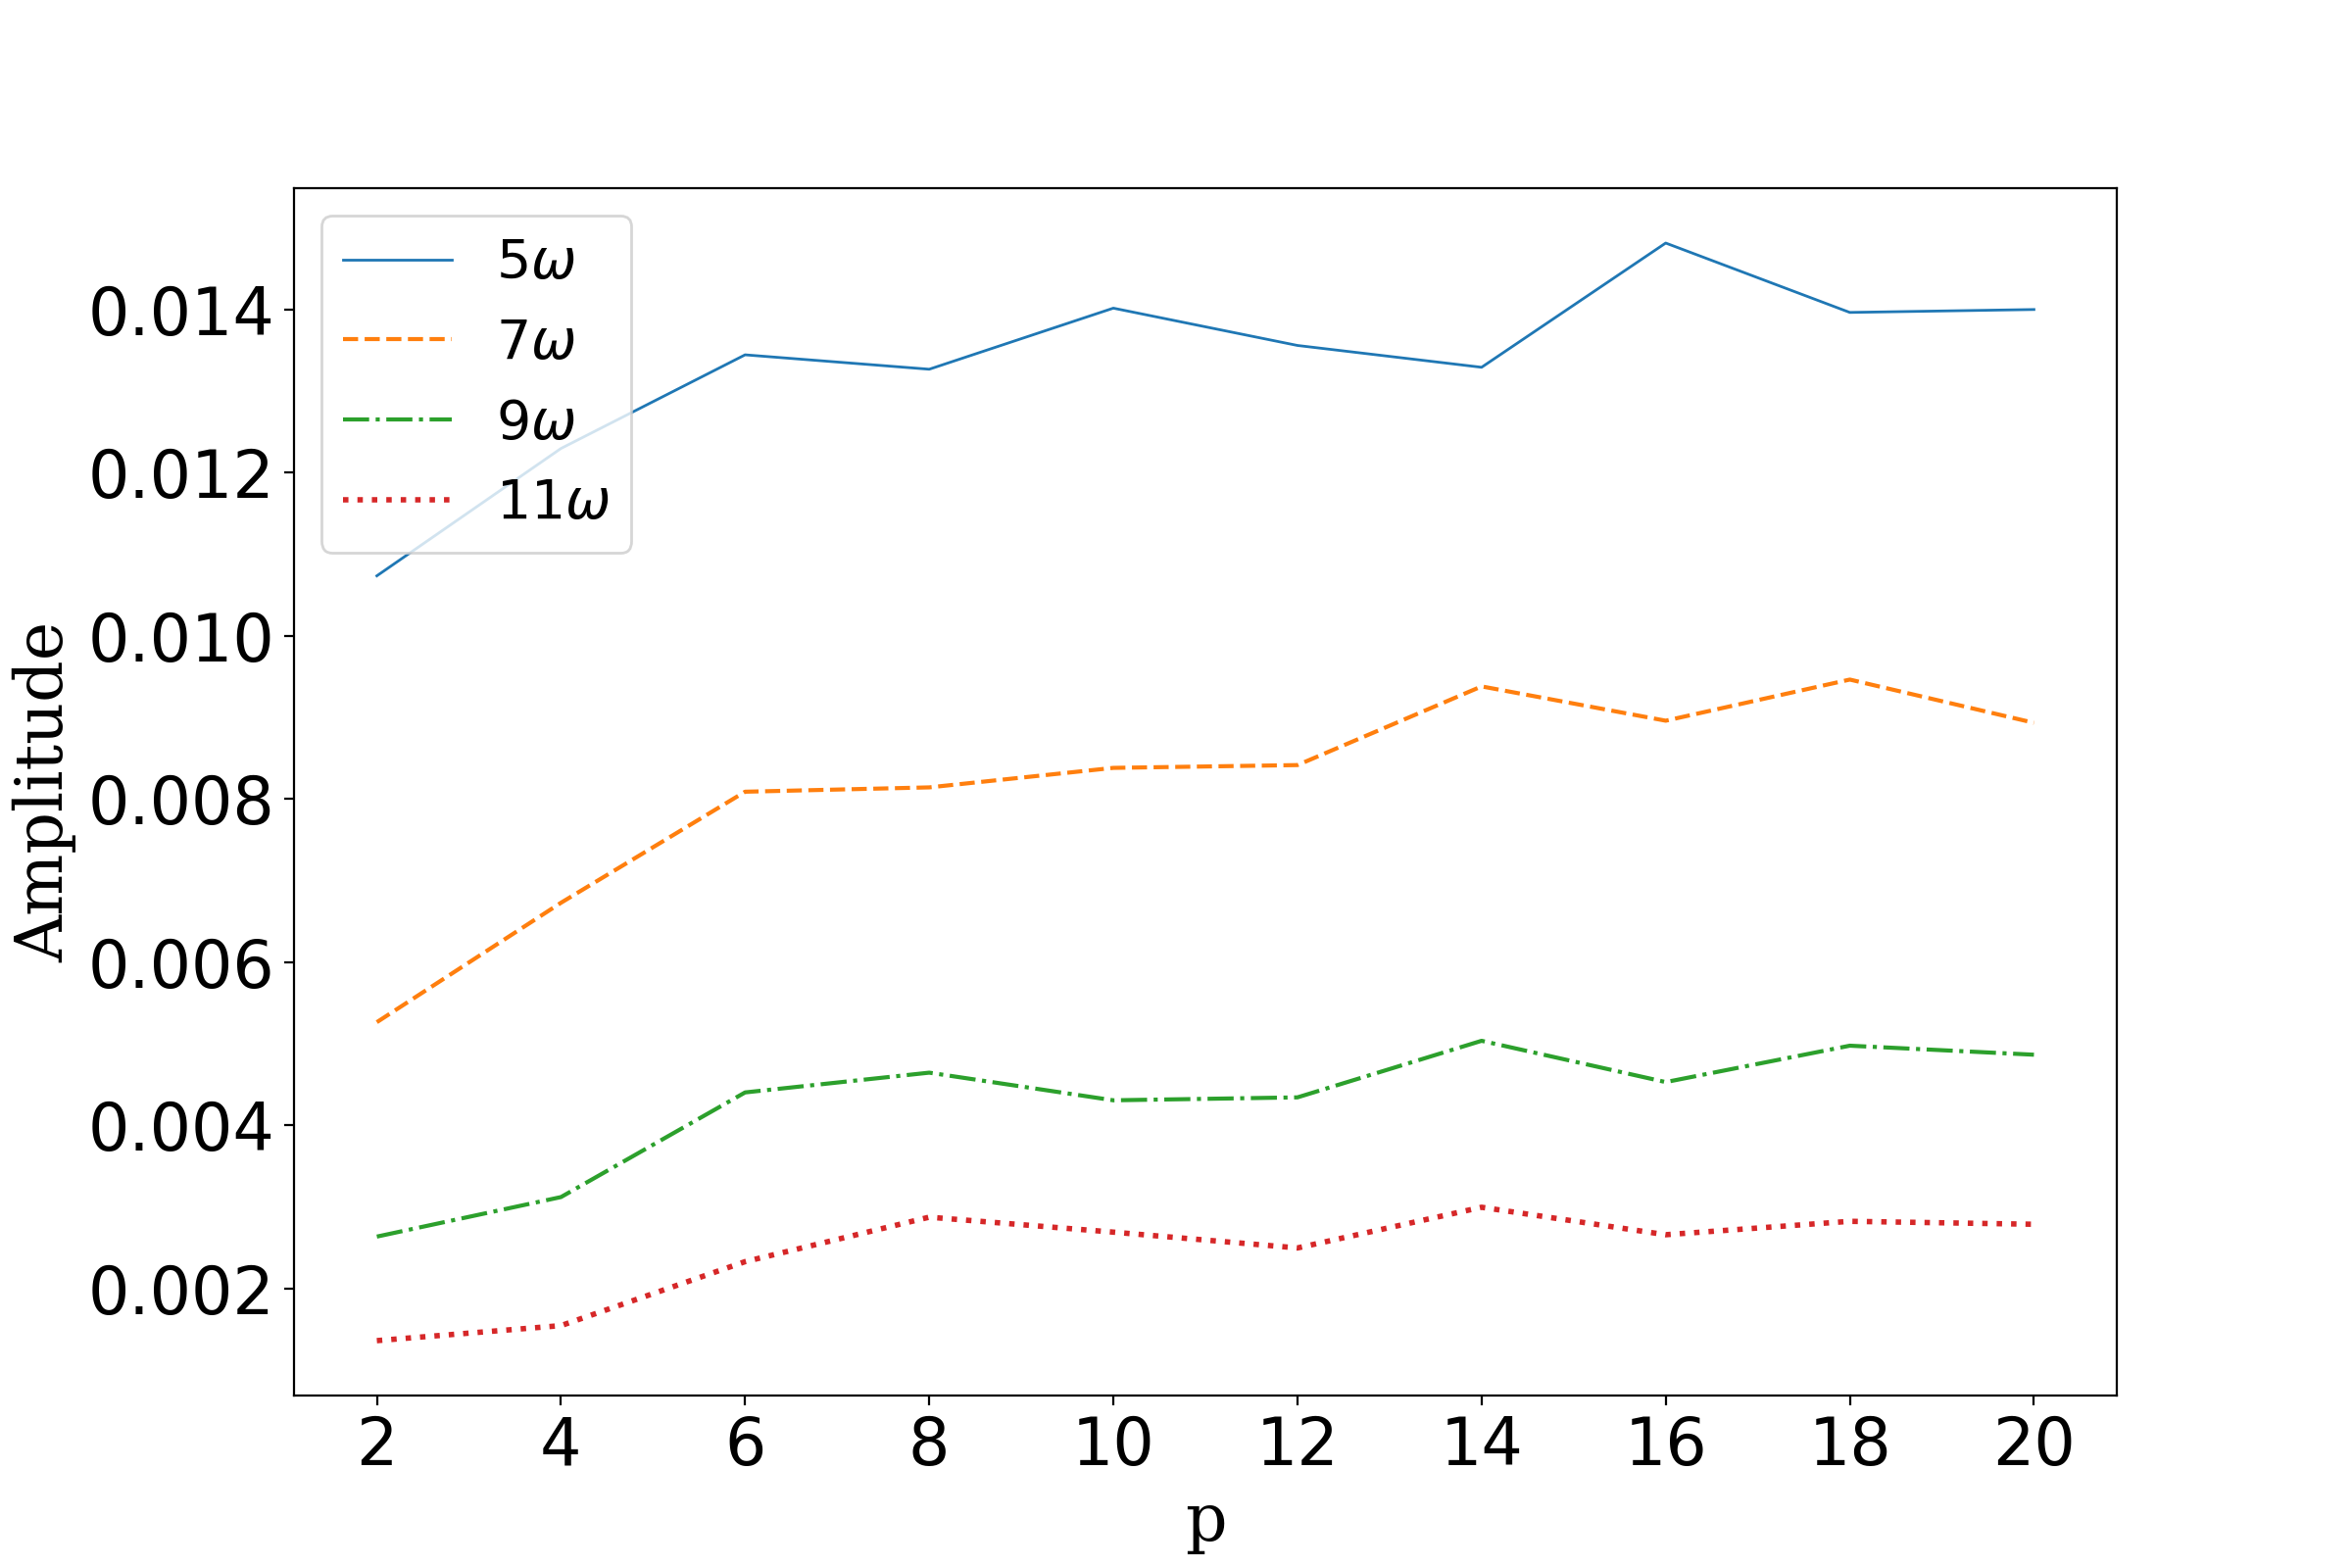
\includegraphics[width=1\textwidth, height=0.60\textheight]{images/SG_peak_amplitude.png}
        \scriptsize{This figure shows the peak amplitude of the HHG as a function of the power of the SG envelope. The peak amplitude increases with increasing power.}
        \label{fig:sg-peak}
    \end{minipage}
\end{frame}

% \begin{frame}
%     \frametitle{Results: p-Polarized Laser}
%     \begin{figure}[h]
%         \centering
%         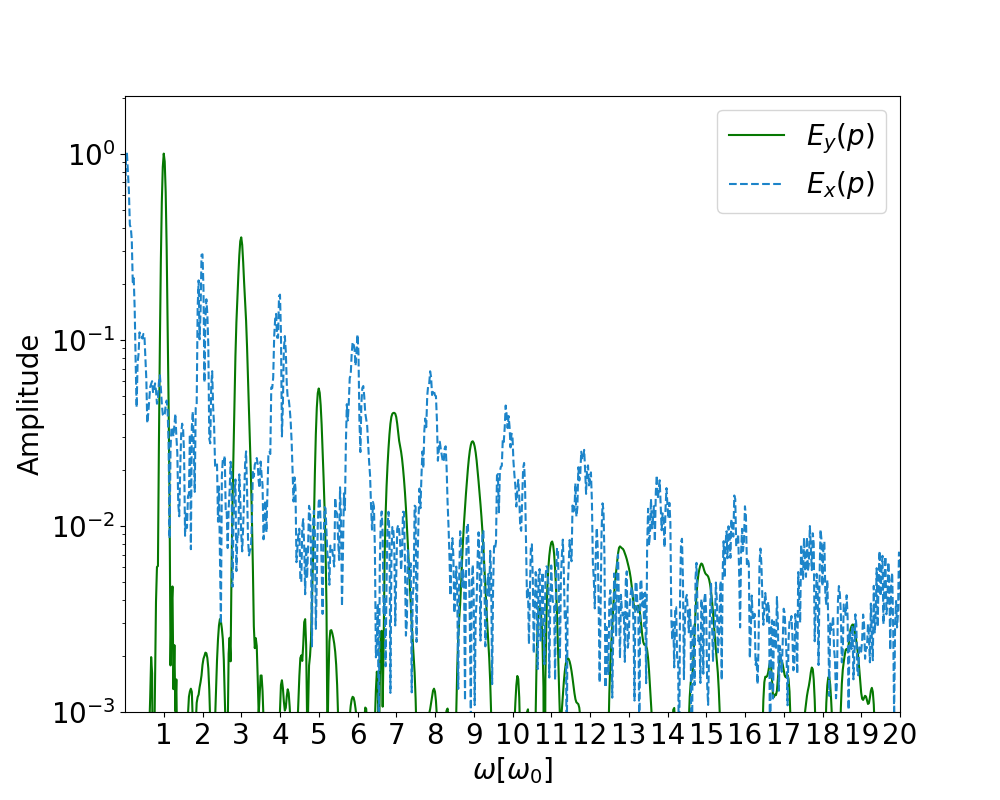
\includegraphics[width=0.75\textwidth]{images/p_fft.png}
%         \caption{\small{Spectrum of HHG for p-polarized light. Simulation parameters are $\alpha = \pi/4$, the density is $n_0 = 7n_c$ and $a_0 = 4$}}
%     \end{figure}
% \end{frame}

% \begin{frame}
%     \frametitle{Results: s-Polarized Laser}
%     \begin{figure}
%         \centering
%         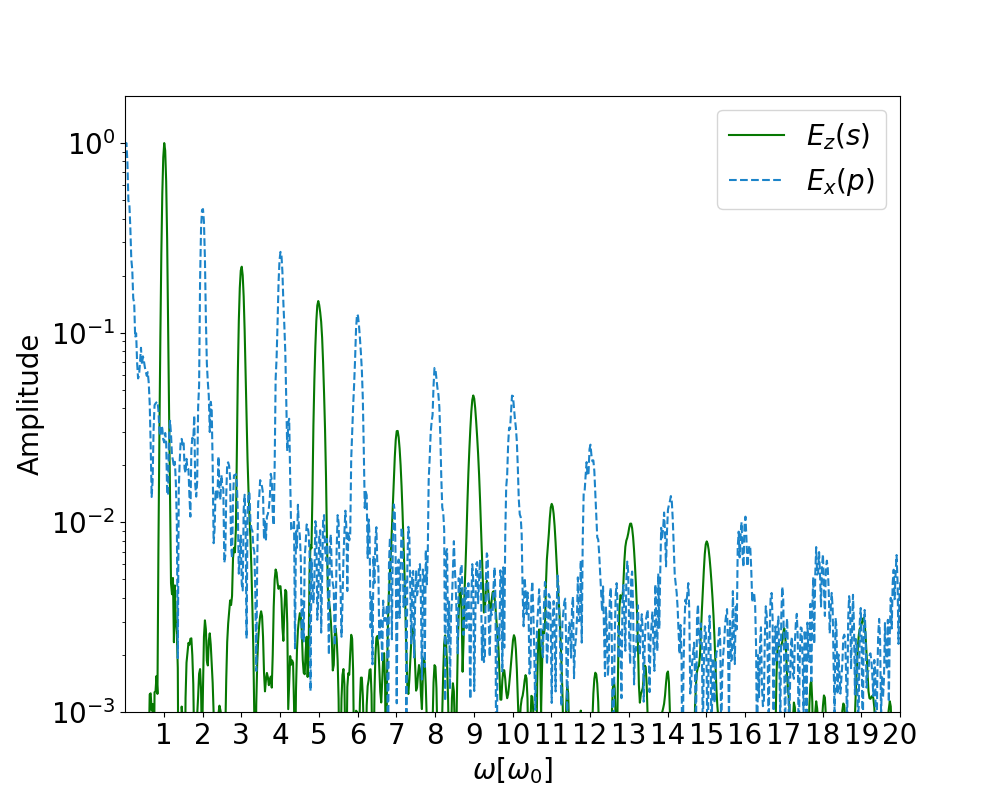
\includegraphics[width=0.75\textwidth]{images/s_fft.png}
%         \caption{\small{Spectrum of HHG for s-polarized light. Simulation parameters are $\alpha = \pi/4$, the density is $n_0 = 7n_c$ and $a_0 = 4$}}
%     \end{figure}
% \end{frame}
\begin{frame}
    \frametitle{Simulation Details: 2D}
    \small
    To compare the results of the 1D oblique incidence using Bourdier transformation, we did some 2D simulations using EPOCH. Most of the simulation parameters are the same.
    % \begin{minipage}[t]{0.48\linewidth}
    %     \begin{itemize}
    %         \item Particles per cell: 100
    %         \item Number of cells: 16000
    %         \item Wavelength $\lambda_l = 1 \mu m$
    %         \item Pulse duration $= 20 \tau$ ($\tau\approx 3.3 fs$)
    %         \item Simulation time $= 40 \tau$
    %         \item Intensity of laser for $a_0 = 0.5$ is $I = 3.425 \times 10^{17} W/cm^2$
    %         \item The density to critical density ratio is $n_0/n_c = 4$
    %     \end{itemize}
    %     We also performed simulations with p- and s-polarized laser incidence at oblique angle.
    % \end{minipage}
    \begin{minipage}[t]{0.64\linewidth}
        \begin{figure}
            \centering
            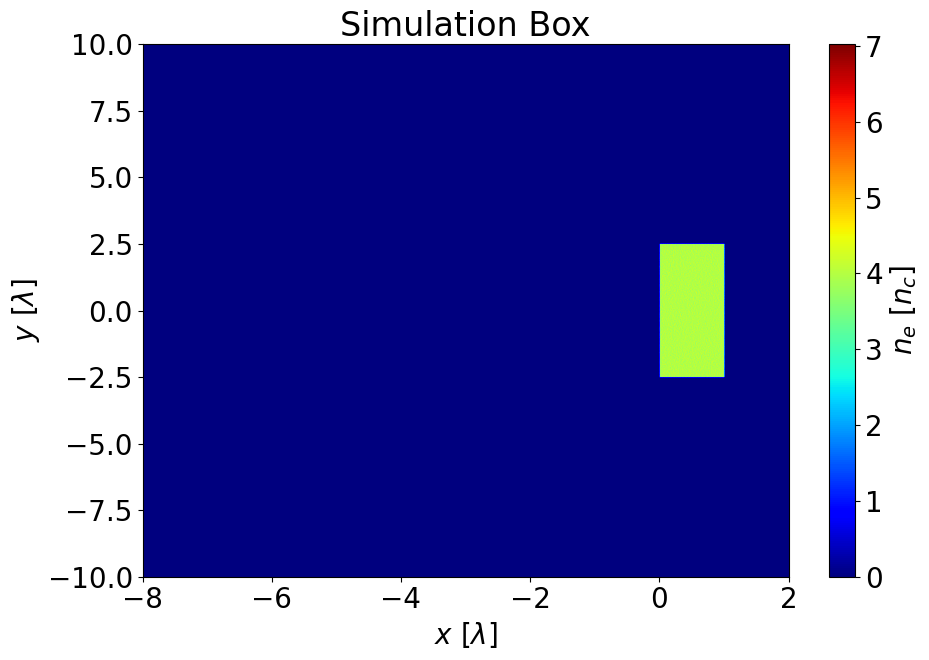
\includegraphics[width=1.0\textwidth, height=0.62\textheight]{images/2dbox.png}
            \label{fig:2dbox}
        \end{figure}
    \end{minipage}
    \begin{minipage}[t]{0.34\linewidth}
        \begin{center}
            \begin{itemize}
                \item Box size has been changed
                \item $N_x = 2000$ and $N_y = 4000$
                \item The pulse width is now $8\tau$
                \item Simulation is run for $30\tau$
            \end{itemize}
        \end{center}
    \end{minipage}
\end{frame}

\begin{frame}
    \frametitle{Results: p- and s-Polarized Laser Using 1D Simulations}
    \begin{minipage}[h]{0.48\linewidth}
        \centering
        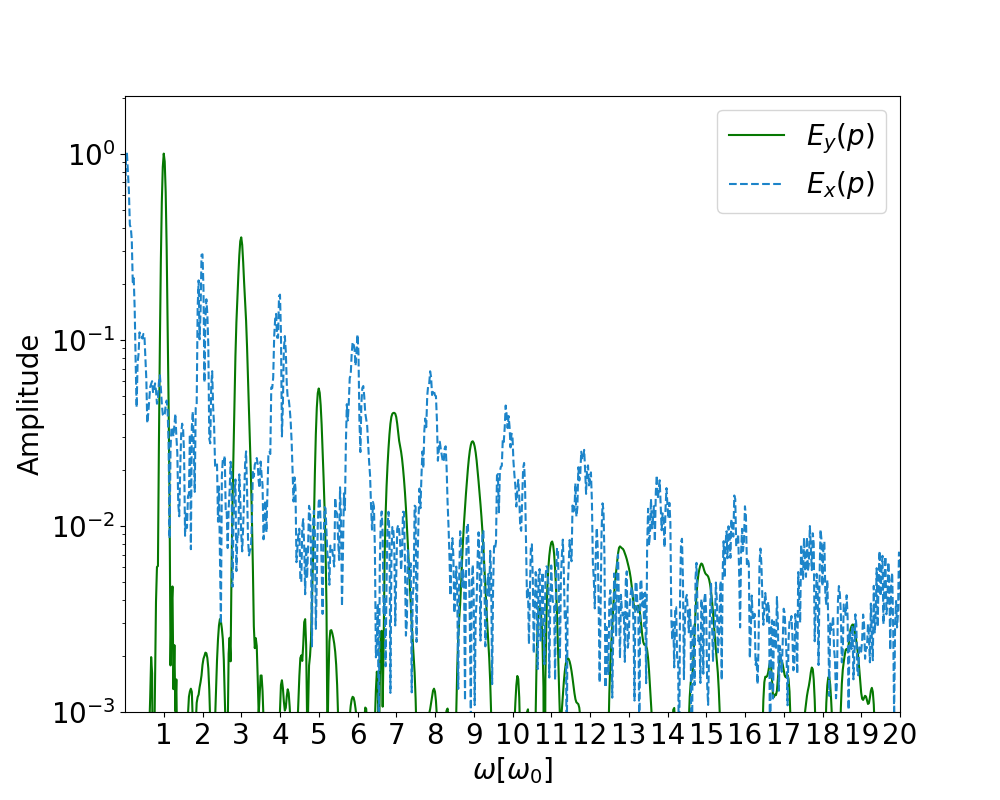
\includegraphics[width=1\textwidth, height=0.60\textheight]{images/p_fft.png}
        \scriptsize{The spectrum of HHG for p-polarized light. Simulation parameters are $\alpha = \pi/4$, the density is $n_0 = 7n_c$ and $a_0 = 4$. We see that $E_x$ gives rise to even harmonics and $E_y$ gives rise to odd harmonics.}
        \label{fig:p-peak}
    \end{minipage}
    \begin{minipage}[h]{0.48\linewidth}
        \centering
        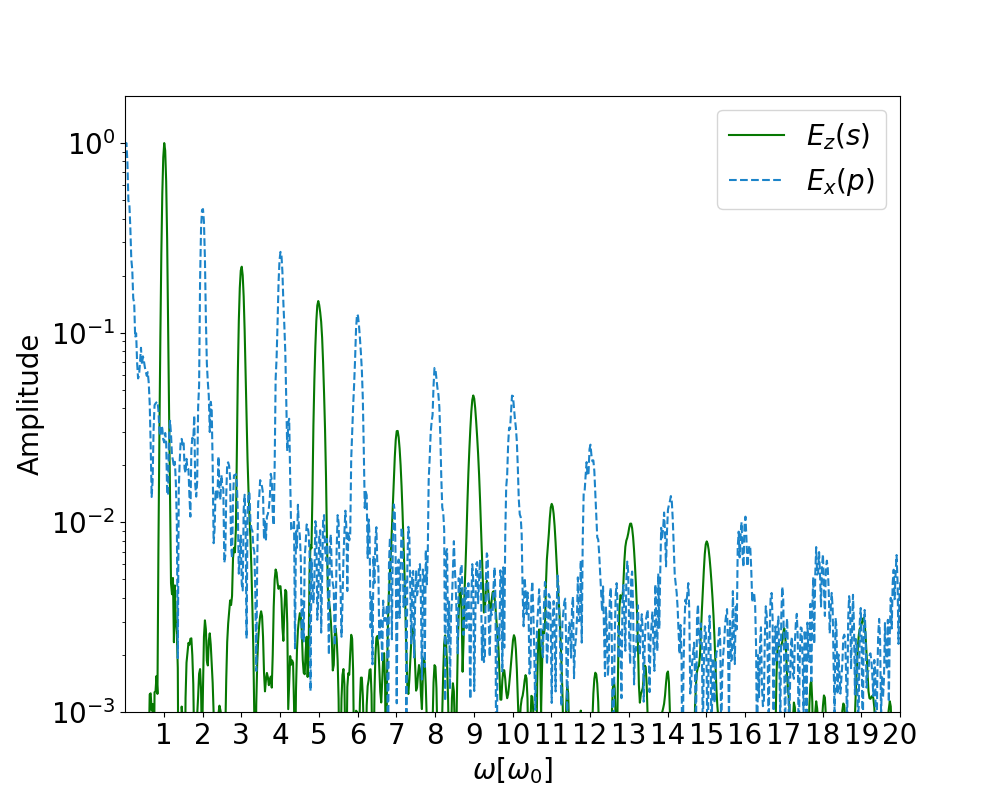
\includegraphics[width=1\textwidth, height=0.60\textheight]{images/s_fft.png}
        \scriptsize{The spectrum of HHG for s-polarized light. Simulation parameters are $\alpha = \pi/4$, the density is $n_0 = 7n_c$ and $a_0 = 4$. Here s-polarized odd and p-polarized even harmonics are generated.}
        \label{fig:s-fft}
    \end{minipage}
    %     \begin{figure}[h]
    %         \centering
    %         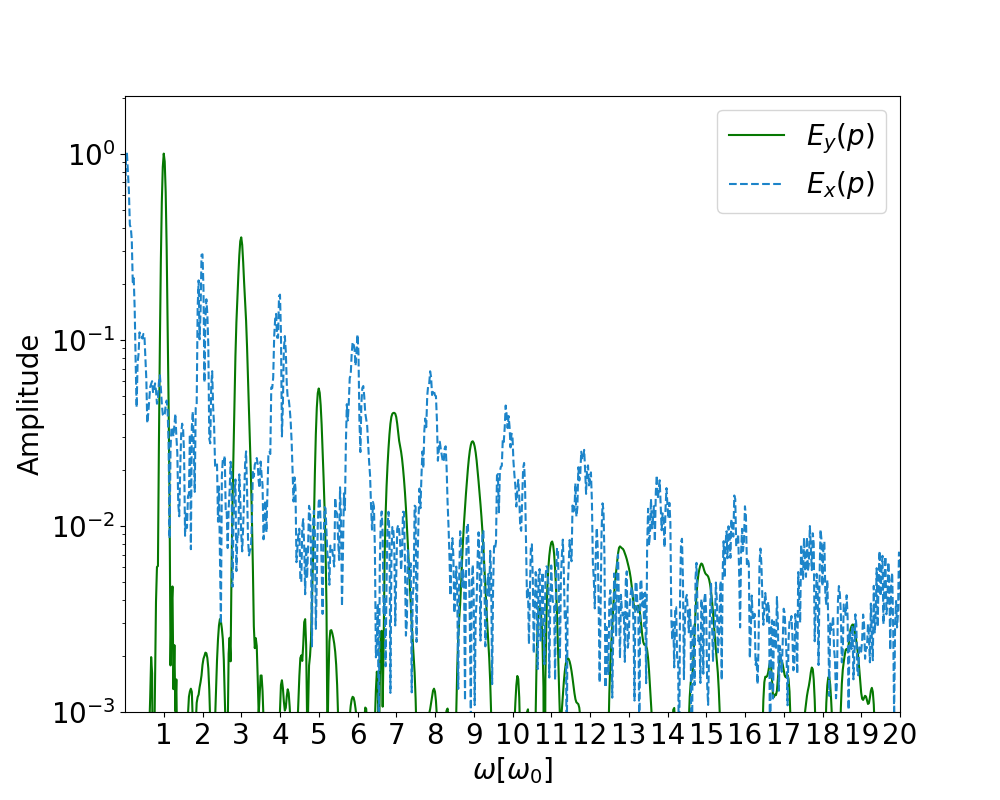
\includegraphics[width=0.75\textwidth]{images/p_fft.png}
    %         \caption{\small{Spectrum of HHG for p-polarized light. Simulation parameters are $\alpha = \pi/4$, the density is $n_0 = 7n_c$ and $a_0 = 4$}}
    %     \end{figure}
    % \end{frame}

    % \begin{frame}
    %     \frametitle{Results: s-Polarized Laser}
    %     \begin{figure}
    %         \centering
    %         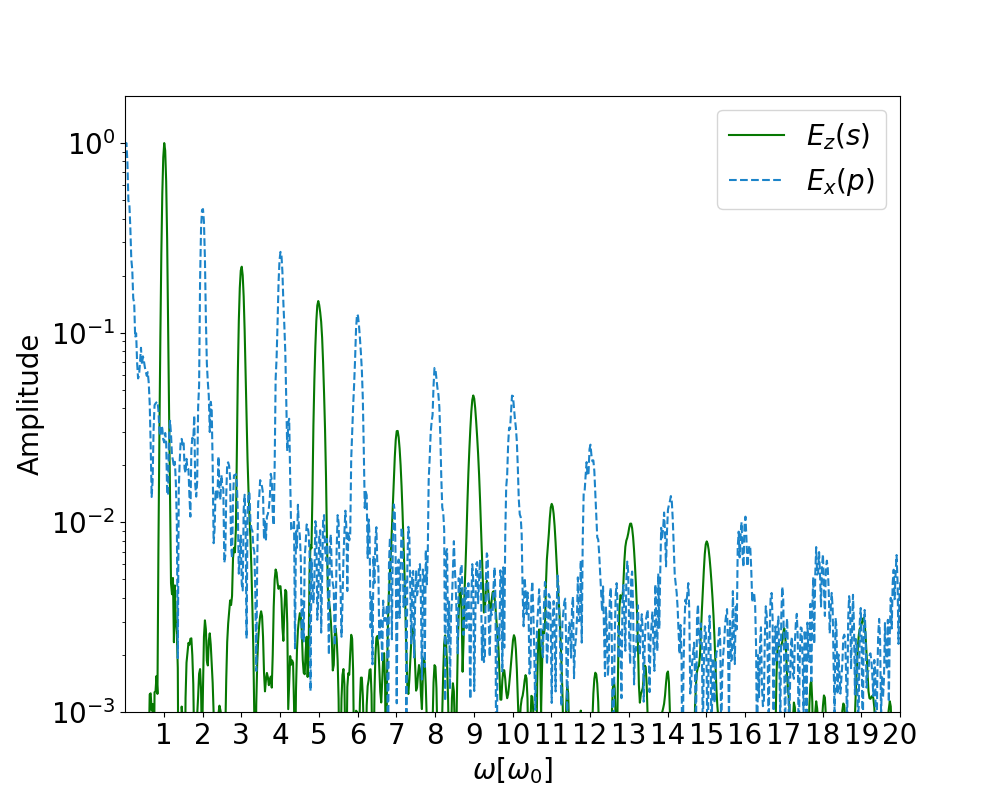
\includegraphics[width=0.75\textwidth]{images/s_fft.png}
    %         \caption{\small{Spectrum of HHG for s-polarized light. Simulation parameters are $\alpha = \pi/4$, the density is $n_0 = 7n_c$ and $a_0 = 4$}}
    %     \end{figure}
\end{frame}

\begin{frame}
    \frametitle{Results: p-Polarized Laser Using 2D Simulations}
    \centering
    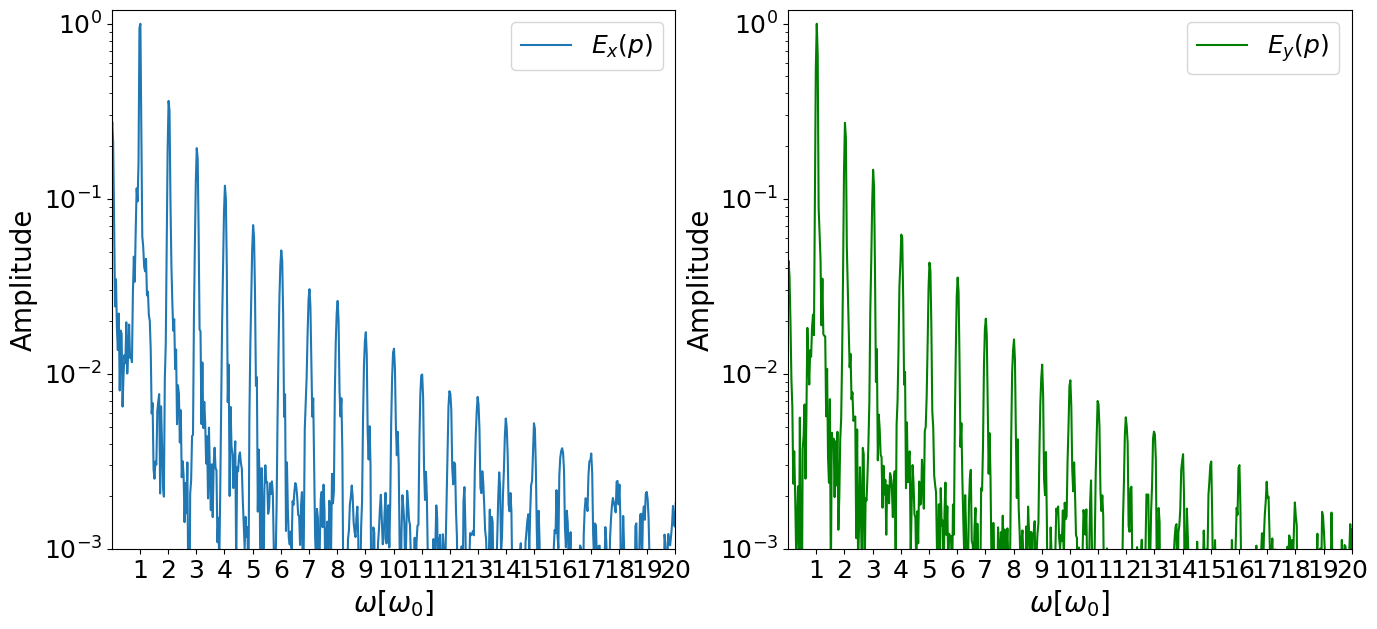
\includegraphics[width=1\textwidth]{images/p2d.png}
    \scriptsize{The spectrum shows that both $E_x$ and $E_y$ has odd as well as even harmonics, in contrast with the 1D case. $E_z$ is zero. Simulation parameters are $\alpha = \pi/4$, the density is $n_0 = 7n_c$ and $a_0 = 4$.}
    \label{fig:p2d}
\end{frame}

\begin{frame}
    \frametitle{Results: s-Polarized Laser Using 2D Simulations}
    \centering
    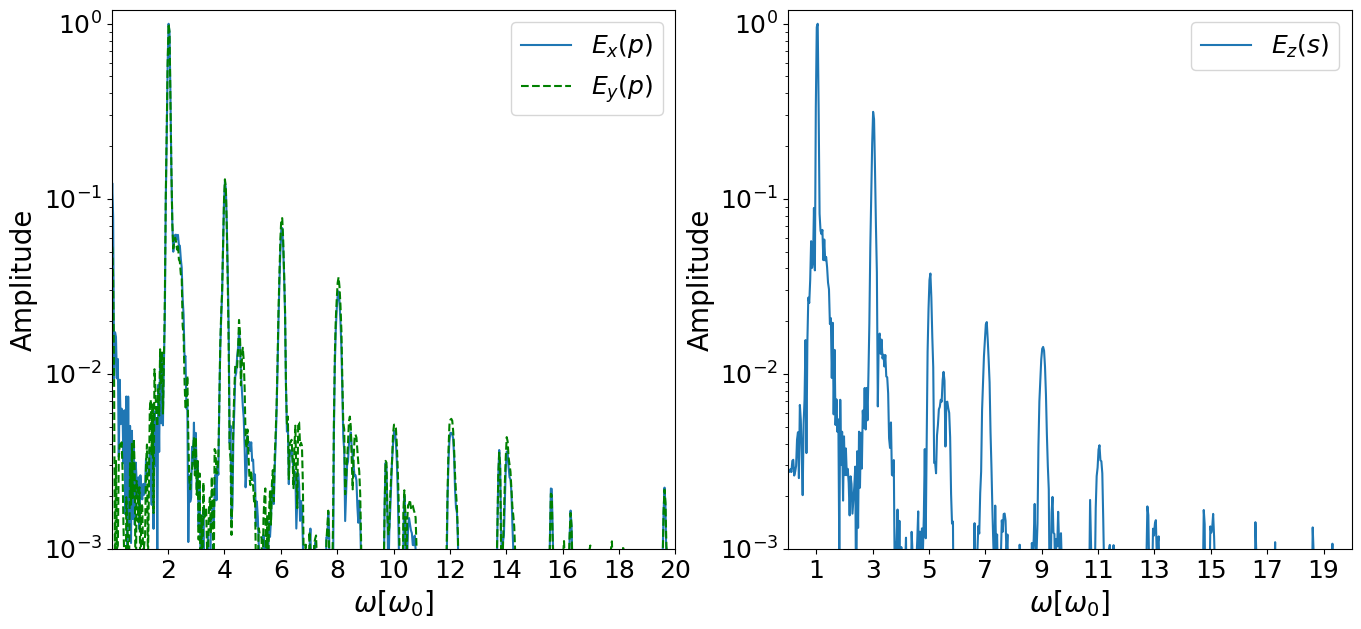
\includegraphics[width=1\textwidth]{images/s2d.png}
    \scriptsize{Fields $E_x$ and $E_y$ has even harmonics, as expected by the selection rule. $E_z$ has odd harmonics. This time, results are similar to the 1D case. Simulation parameters are $\alpha = \pi/4$, the density is $n_0 = 7n_c$ and $a_0 = 4$.}
    \label{fig:s2d}
\end{frame}

\begin{frame}
    \frametitle{Current Status and Future Scope}
    \small
    \textbf{Current Status}
    \begin{itemize}
        \item Presence of pre-plasma reduces the quality of HHG generated.
        \item SG envelopes results in a small shift in peak amplitudes.
        \item For p-polarized laser, even and odd p-polarized harmonics.
        \item For s-polarized laser, odd s-polarized harmonics and even p-polarized harmonics.
    \end{itemize}
    \textbf{Future Scope}
    \begin{itemize}
        \item Study oblique incidence and polarization more rigorously.
        \item Do 2D simulations.
        \item Compare it with the 1D results.
    \end{itemize}
    \textbf{Acknowledgement}
    We would like to extend our sincerest gratitude to Professor Vikrant Saxena for his unwavering support, patience, motivation, enthusiasm, and invaluable guidance.
\end{frame}
\end{document}